\documentclass{beamer} 
\usepackage{amsmath,amsthm,amsfonts}
\usepackage{graphicx,microtype,parskip}
\usepackage{caption,subcaption,multirow}
\usepackage{attrib}

\frenchspacing

\usetheme{default}
\usecolortheme{whale}

\setbeamertemplate{navigation symbols}{}

\setbeamercolor{title}{fg=blue,bg=white}

\setbeamercolor{block title}{fg=white,bg=gray}
\setbeamercolor{block body}{fg=black,bg=lightgray}

\setbeamercolor{block title alerted}{fg=white,bg=darkgray}
\setbeamercolor{block body alerted}{fg=black,bg=lightgray}

\let\Tiny\tiny% http://tex.stackexchange.com/q/58087/5764

\setbeamertemplate{footline} {
  \hbox{\begin{beamercolorbox}[wd=1\paperwidth,ht=2.25ex,dp=1ex,right]{framenumber}%
    \usebeamerfont{framenumber}\insertframenumber{} / \inserttotalframenumber\hspace*{2ex}
  \end{beamercolorbox}}%
  \vskip0pt%
}

\AtBeginSection[]
{
  \begin{frame}
    \tableofcontents[currentsection]
  \end{frame}
}
\AtBeginSubsection[]
{
  \begin{frame}
    \tableofcontents[currentsection,currentsubsection]
  \end{frame}
}


\title{Remodeling the fossil record}
\subtitle{analysis of emergent evolutionary and ecological patterns}
\author{Peter D Smits}
\institute{Committee on Evolutionary Biology, University of Chicago}
\titlegraphic{
  
\includegraphics[width=2.75cm,height=2.75cm,keepaspectratio=true]{figure/paleodb}
  \hspace*{0.35\paperwidth}
  
\includegraphics[width=2cm,height=2cm,keepaspectratio=true]{figure/chicago}
}
\date{}

\begin{document}

\begin{frame}
  \maketitle
\end{frame}

\begin{frame}
  \tableofcontents
\end{frame}

\section{Macroevolution and macroecology}

\begin{frame}
  \begin{columns}
    \begin{column}{0.5\textwidth}
      \begin{center}
        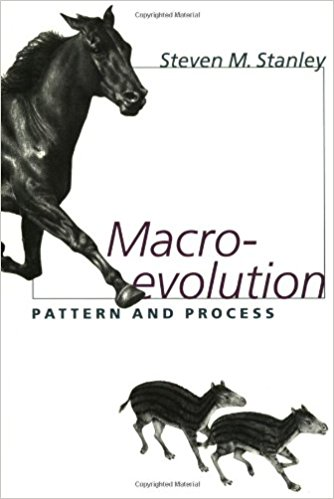
\includegraphics[height=0.8\textheight,width=\textwidth,keepaspectratio=true]{figure/stanley_macro}
      \end{center}
    \end{column}
    \begin{column}{0.5\textwidth}
      \begin{center}
        
\includegraphics[height=0.8\textheight,width=\textwidth,keepaspectratio=true]{figure/brown_macro}
      \end{center}
    \end{column}
  \end{columns}
\end{frame}

\begin{frame}
  \begin{definition}
    \begin{itemize}
      \item \alert{macroevolution}: study of patterns which emerge when considering the evolutionary history of multiple species.
      \item \alert{macroecology}: study of patterns which emerge when considering the ecology of multiple species.
      \item \emph{in both time and space}
    \end{itemize}
  \end{definition}
\end{frame}

\begin{frame}
  \frametitle{Traits as conceptual and operational link}

  \begin{definition}
    \begin{itemize}
      \item \alert{trait}: identifiable property of an organism \\e.g. pelage color, body mass, beak depth, tooth shape
      \item \alert{functional trait}: trait that strongly influences performance/means of interacting with environment
      \item \alert{species trait}: identifiable property assignable to a species
    \end{itemize}
  \end{definition}
\end{frame}

\begin{frame}
  \frametitle{Species selection}

  \begin{alertblock}{Rabosky and McCune 2010 \em{TREE}}
    \begin{quote}
      Species selection is the outcome of heritable variation in speciation and extinction rates among taxa.
    \end{quote}
  \end{alertblock}

  \begin{itemize}
    \item avoids selection versus sorting, ``strict'' species selection versus effect macroevolution
  \end{itemize}
\end{frame}

\begin{frame}
  \frametitle{Species fitness}

  \begin{alertblock}{Cooper 1984 \em{J. Theoretical Biology}}
    Expected time till extinction.
  \end{alertblock}


  \begin{itemize}
    \item \alert{logic:} if more fit, more likely to be present
    \item distribution based definition (population)
    \item other definitions can be derived based on definition of extinction
  \end{itemize}

\end{frame}

\begin{frame}
  \frametitle{Extinction}


  \begin{block}{Simpson 2016 \em{bioRxiv}}
    \begin{quote}
      Population decline maybe a common cause of \dots extinction, but organisms never die from population decline, and population decline is never caused by organismal death alone \dots It's the relative balance between birth, death, and lifespan of organisms that determines \dots extinction. 
    \end{quote}
  \end{block}

\end{frame}

\begin{frame}
  \frametitle{Law of Constant Extinction}

  \begin{alertblock}{Van Valen 1973 \em{Evol. Theory}}
    Extinction risk, in a given adaptive zone, is taxon--age independent.
  \end{alertblock}

\end{frame}

\begin{frame}
  \frametitle{Survival of the unspecialized}
  \begin{alertblock}{Simpson 1944 \em{Tempo and Mode in Evolution} p. 143}
    \begin{quote}
      When related phyla die out \dots more specialized phyla tend to become extinct before less specialized. This phenomenon is also far from universal, but it is so common that it does deserve recognition as a rule or principle in evolutionary studies: \textbf{the rule of the survival of the relatively unspecialized.}
    \end{quote}
  \end{alertblock}

\end{frame}


\begin{frame}
  \frametitle{Species pool concept}

  \begin{center}
    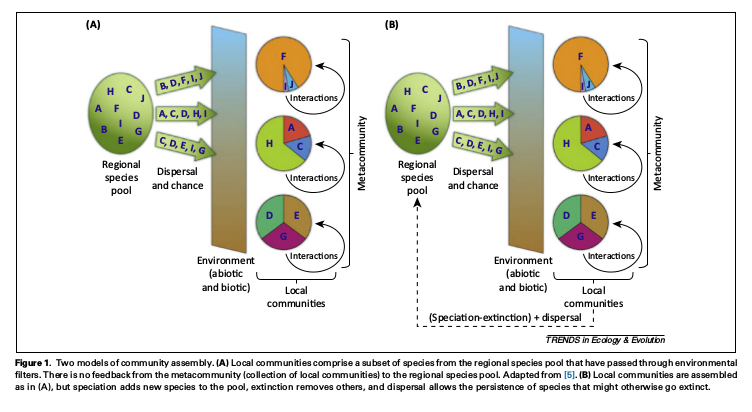
\includegraphics[height=0.8\textheight,width=\textwidth,keepaspectratio=true]{figure/schemske_pool}
  \end{center}

  \tiny{\attrib{Mittelbach and Schemske 2015 \em{TREE}}}
\end{frame}

\begin{frame}
  \frametitle{Functional groups}

  \begin{center}
    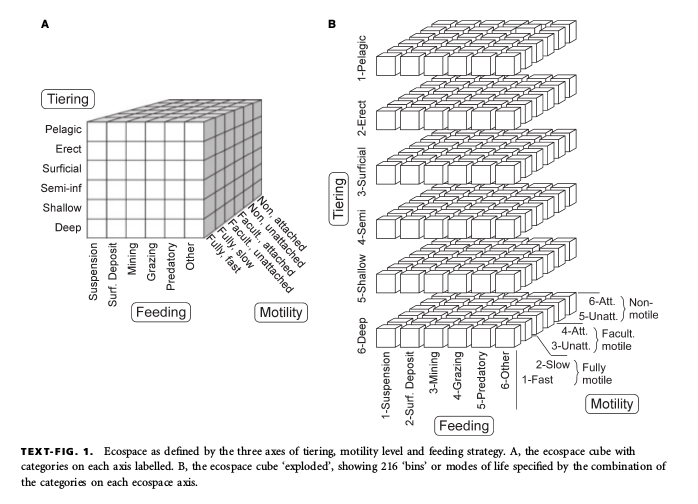
\includegraphics[height=0.8\textheight,width=\textwidth,keepaspectratio=true]{figure/ecocube}
  \end{center}

  \tiny{\attrib{Bambach \em{et al.} 2007 \em{Palaeontology}}}
\end{frame}

\begin{frame}
  \frametitle{Functional groups over time}

  \begin{center}
    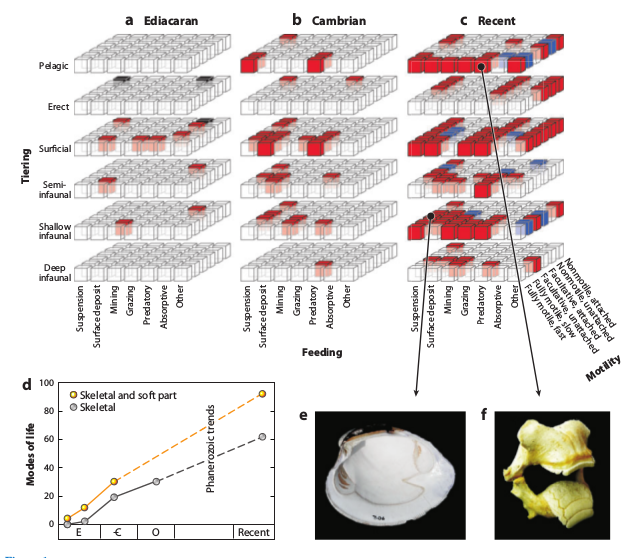
\includegraphics[height=0.8\textheight,width=\textwidth,keepaspectratio=true]{figure/bush_cube_time}
  \end{center}

  \tiny{\attrib{Bush and Bambach 2011 \em{Annu. Rev. Earth Planet Sci.}}}
\end{frame}



\section{Structured data and modelling emergent patterns}

\begin{frame}
  \frametitle{Inference}
  \begin{columns}
    \begin{column}{0.45\textwidth}
      \begin{center}
        
\includegraphics[width = \textwidth,height = 0.8\textheight,keepaspectratio = true]{figure/jaynes_theory}
      \end{center}
    \end{column}
    \begin{column}{0.55\textwidth}
      \begin{quote}
        The theory of probability is the only mathematical tool available to help map the unknown and the uncontrollable.
      \end{quote}
      \tiny{\attrib{Mandelbrot}}
    \end{column}
  \end{columns}
\end{frame}

\begin{frame}
  \frametitle{Structured data in biology and paleontology}

  \begin{center}
    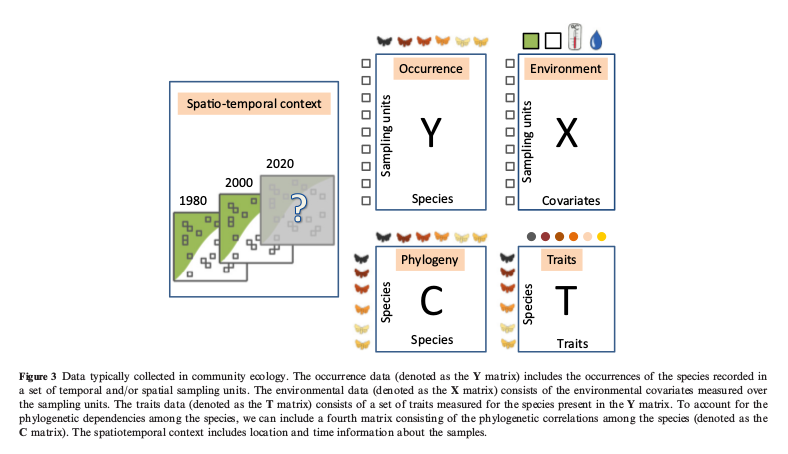
\includegraphics[width = \textwidth,height = 0.8\textheight,keepaspectratio = true]{figure/ovaskainen_data}
  \end{center}

  \tiny{\attrib{Ovaskainen \textit{et al.} 2017 \em{Ecology Letters}}}
\end{frame}

\begin{frame}
  \frametitle{Models of structured data}

  \begin{center}
    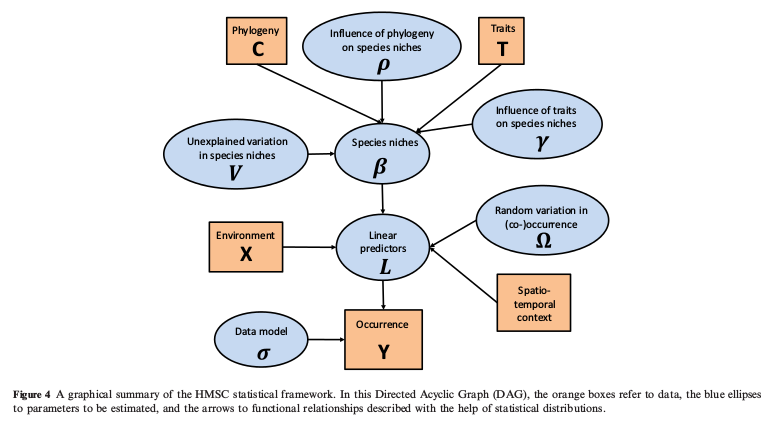
\includegraphics[width = \textwidth,height = 0.8\textheight,keepaspectratio = true]{figure/ovaskainen_dag}
  \end{center}

  \tiny{\attrib{Ovaskainen \textit{et al.} 2017 \em{Ecology Letters}}}
\end{frame}

\begin{frame}
  \frametitle{Models of macroevolution: birth-death}

  \begin{center}
    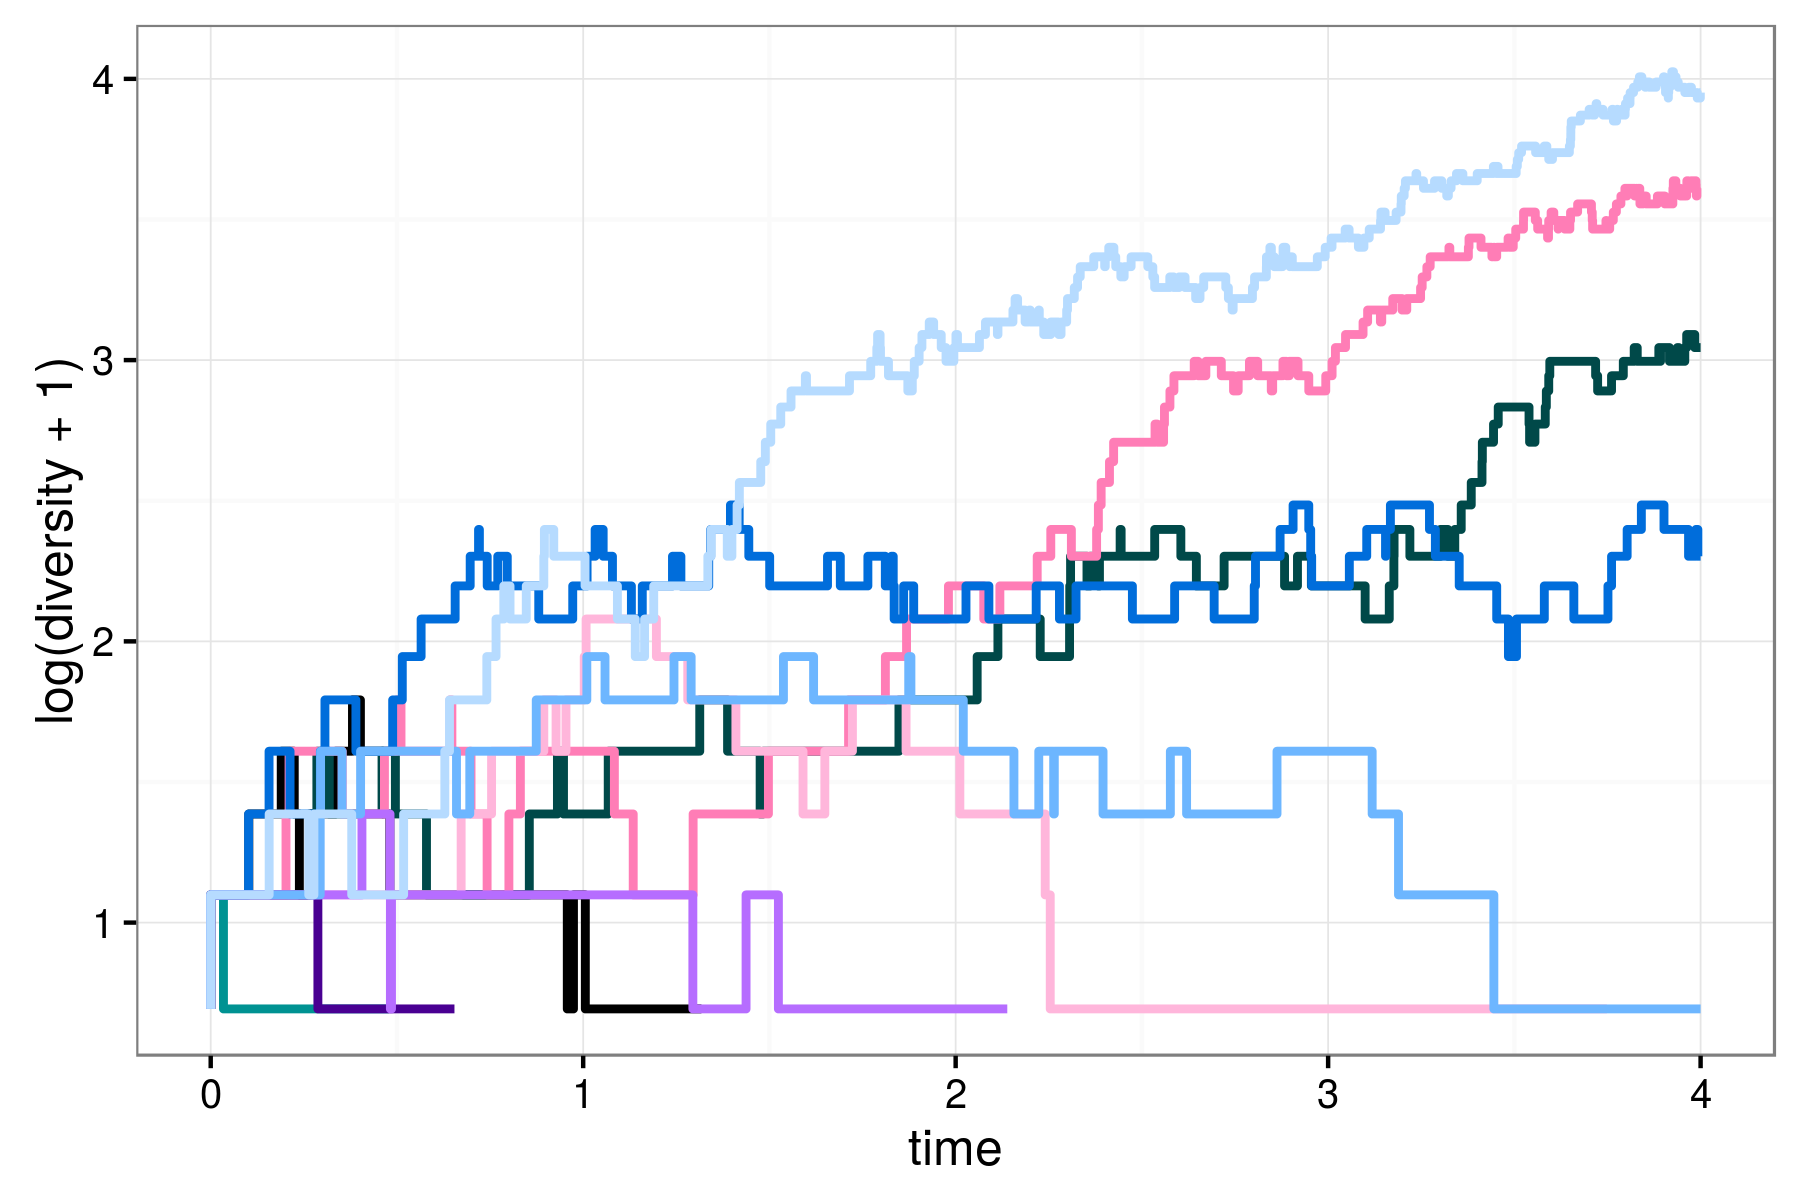
\includegraphics[width = \textwidth,height = 0.7\textheight,keepaspectratio = true]{figure/bd_sim}

    \(m_{t} = a e^{(\lambda - \mu) t}\)
  \end{center}

\end{frame}

\begin{frame}
  \frametitle{Models of macroevolution: Brownian motion}

  \begin{center}
    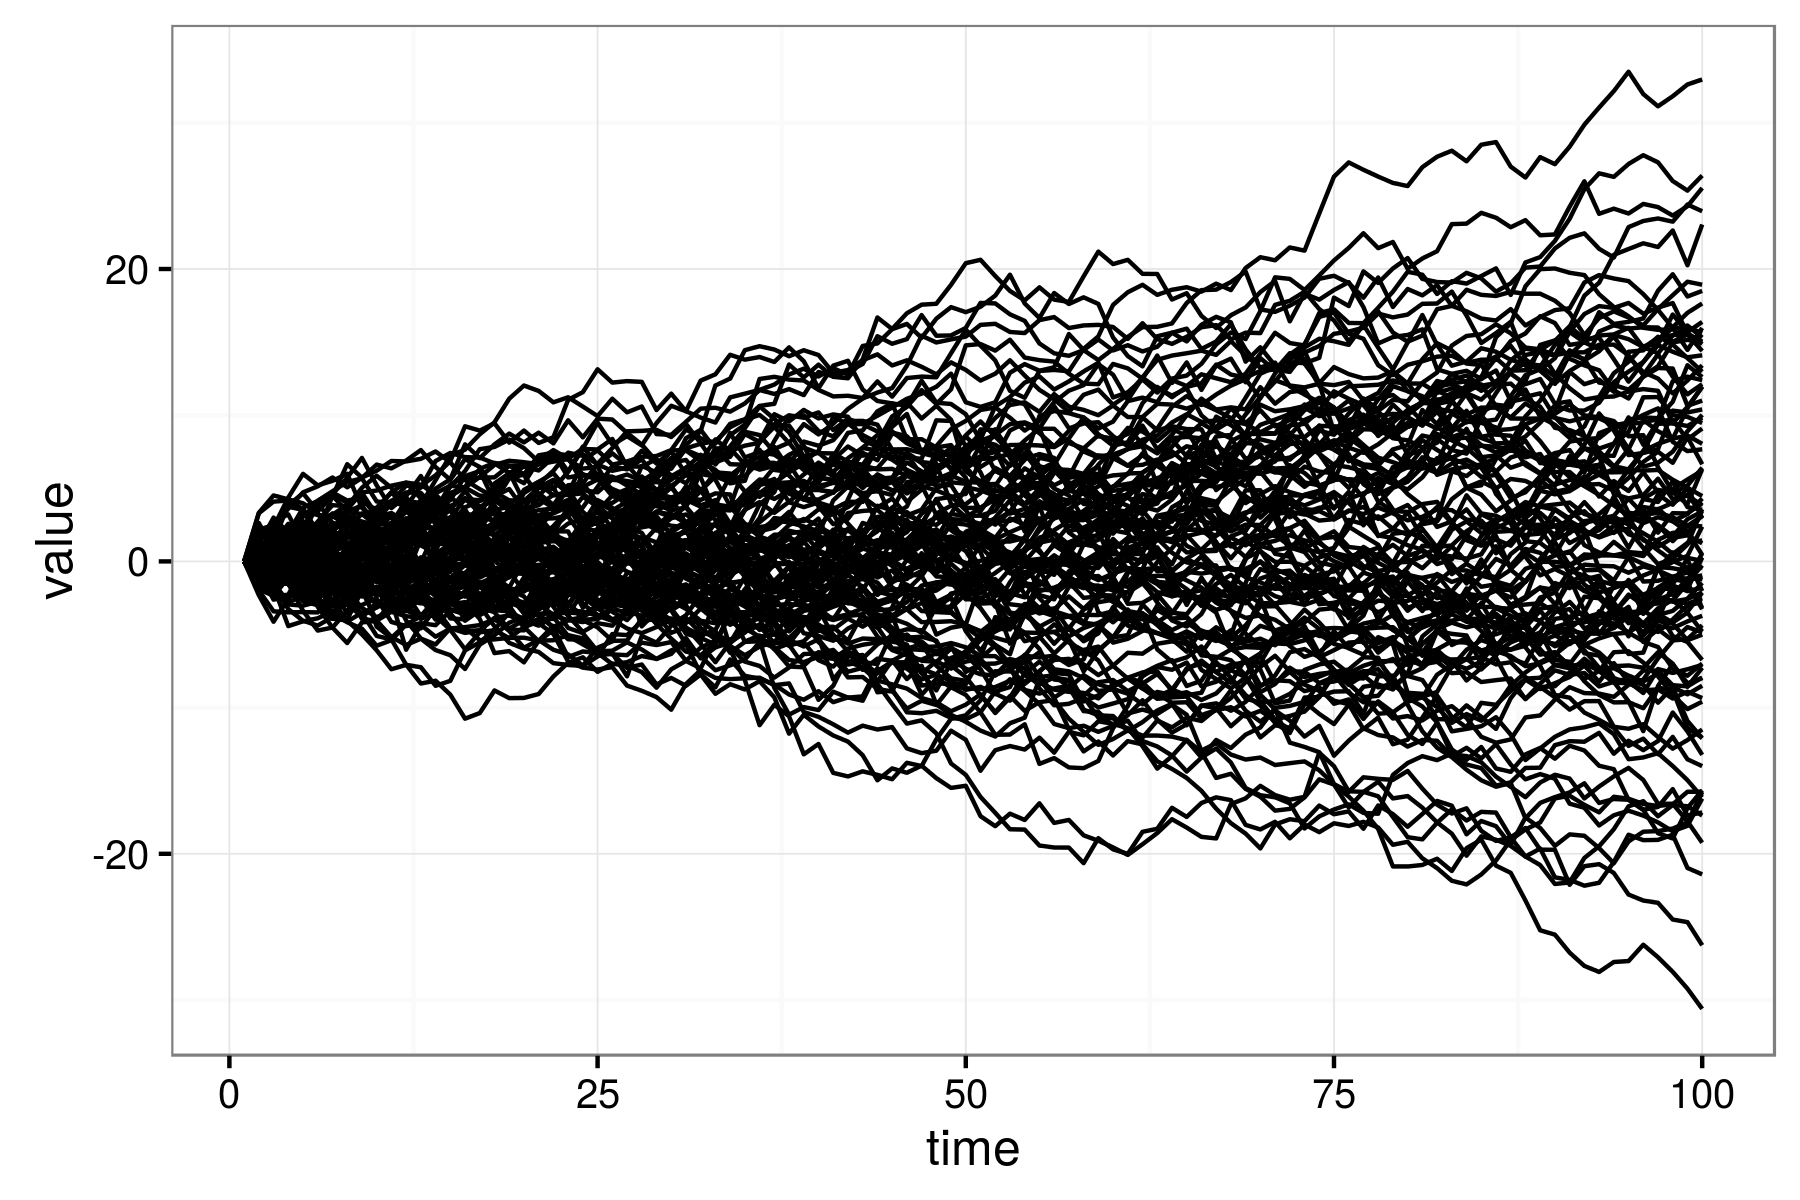
\includegraphics[width = \textwidth,height = 0.7\textheight,keepaspectratio = true]{figure/brown_sim}

    \(x_{t} - x_{s} \sim \mathcal{N}(\mu, \sigma)\)
  \end{center}

\end{frame}


\begin{frame}
  \frametitle{Models of macroecology: species distribution models}

  \begin{columns}
    \begin{column}{0.5\textwidth}
      \begin{block}{Goal}
        Understand species distribution in space (and time) as function of that species' environmental context or species trait values.
      \end{block}
    \end{column}
    \begin{column}{0.5\textwidth}
      \begin{center}
        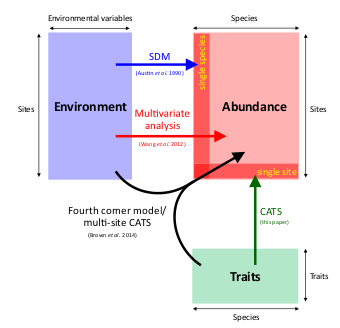
\includegraphics[width = \textwidth,height = 0.5\textheight,keepaspectratio = true]{figure/warton_corner_models}
      \end{center}
    \end{column}
  \end{columns}

  \tiny{\attrib{Warton \textit{et al.} 2015 \em{Methods Ecol. Evol.}}}
\end{frame}

\begin{frame}
  \frametitle{Bayesian statistics}

  \begin{columns}
    \begin{column}{0.5\textwidth}
      \begin{itemize}
        \item Bayesian inference: logic on a continuous scale
        \item flexible, expressive, intuitive
        \item regularize, partial pooling, external information
        \item Stan probabilistic programming language
          \begin{itemize}
            \item Hamiltonian Monte Carlo
            \item Automatic Differentiation Variational Inference
          \end{itemize}
      \end{itemize}
    \end{column}
    \begin{column}{0.5\textwidth}
      \begin{center}
        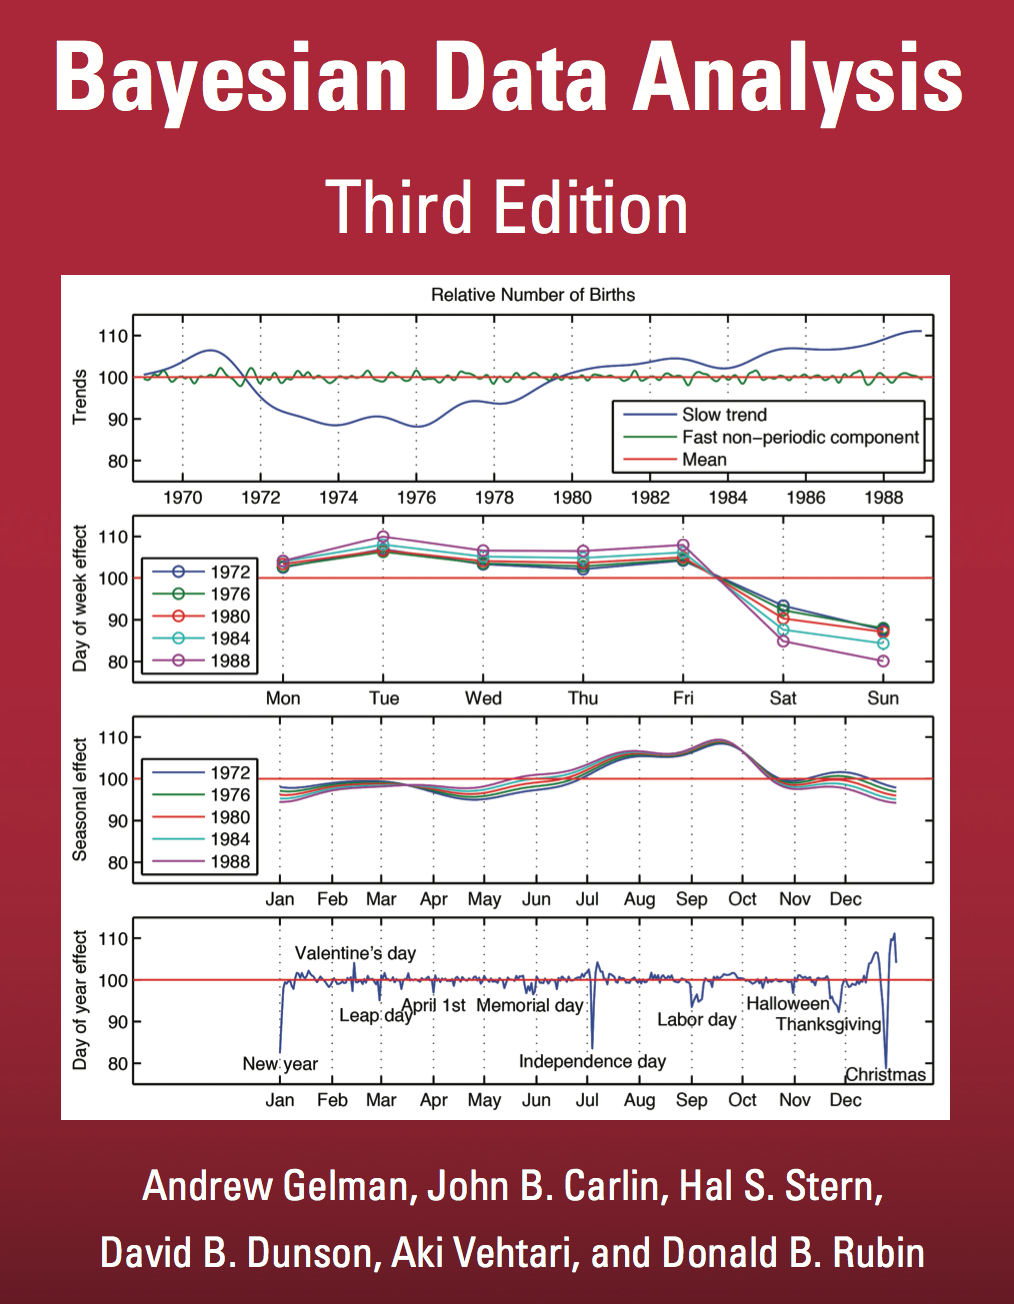
\includegraphics[width = \textwidth,height = 0.8\textheight,keepaspectratio = true]{figure/bda_cover}
      \end{center}
    \end{column}
  \end{columns}
\end{frame}

%\begin{frame}
%  \frametitle{Reading probability as plausibility}
%  \begin{center}
%    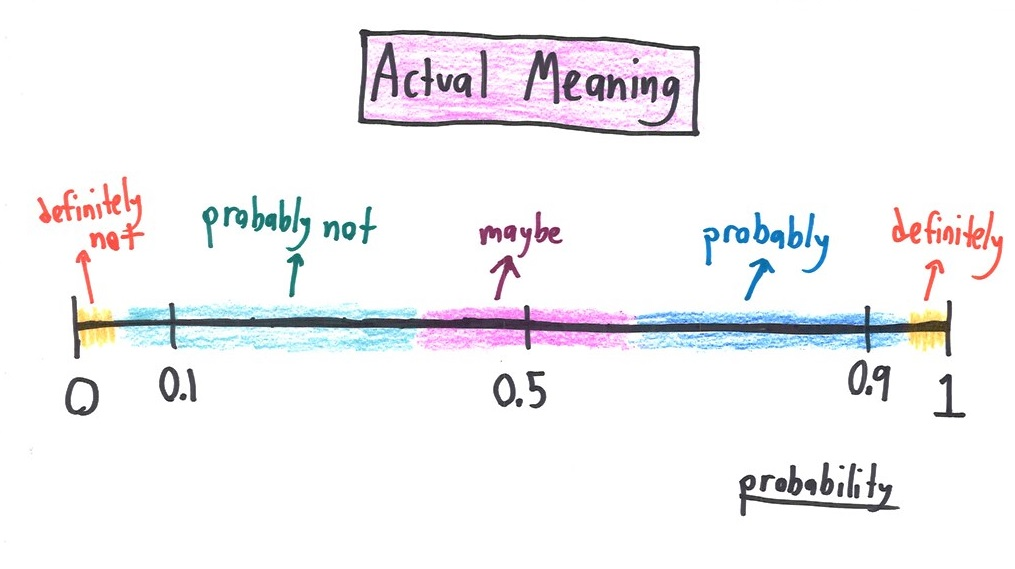
\includegraphics[width = \textwidth,height = 0.8\textheight,keepaspectratio = true]{figure/probability}
%  \end{center}
%
%  \tiny{\attrib{mathwithbaddrawings.com}}
%\end{frame} % opportunity for jokes




\begin{frame}
  \frametitle{Mammals and brachiopods}

  \begin{columns}
    \begin{column}{0.5\textwidth}
      \begin{center}
        \textbf{Mammals}

        \vspace{0.5cm}

        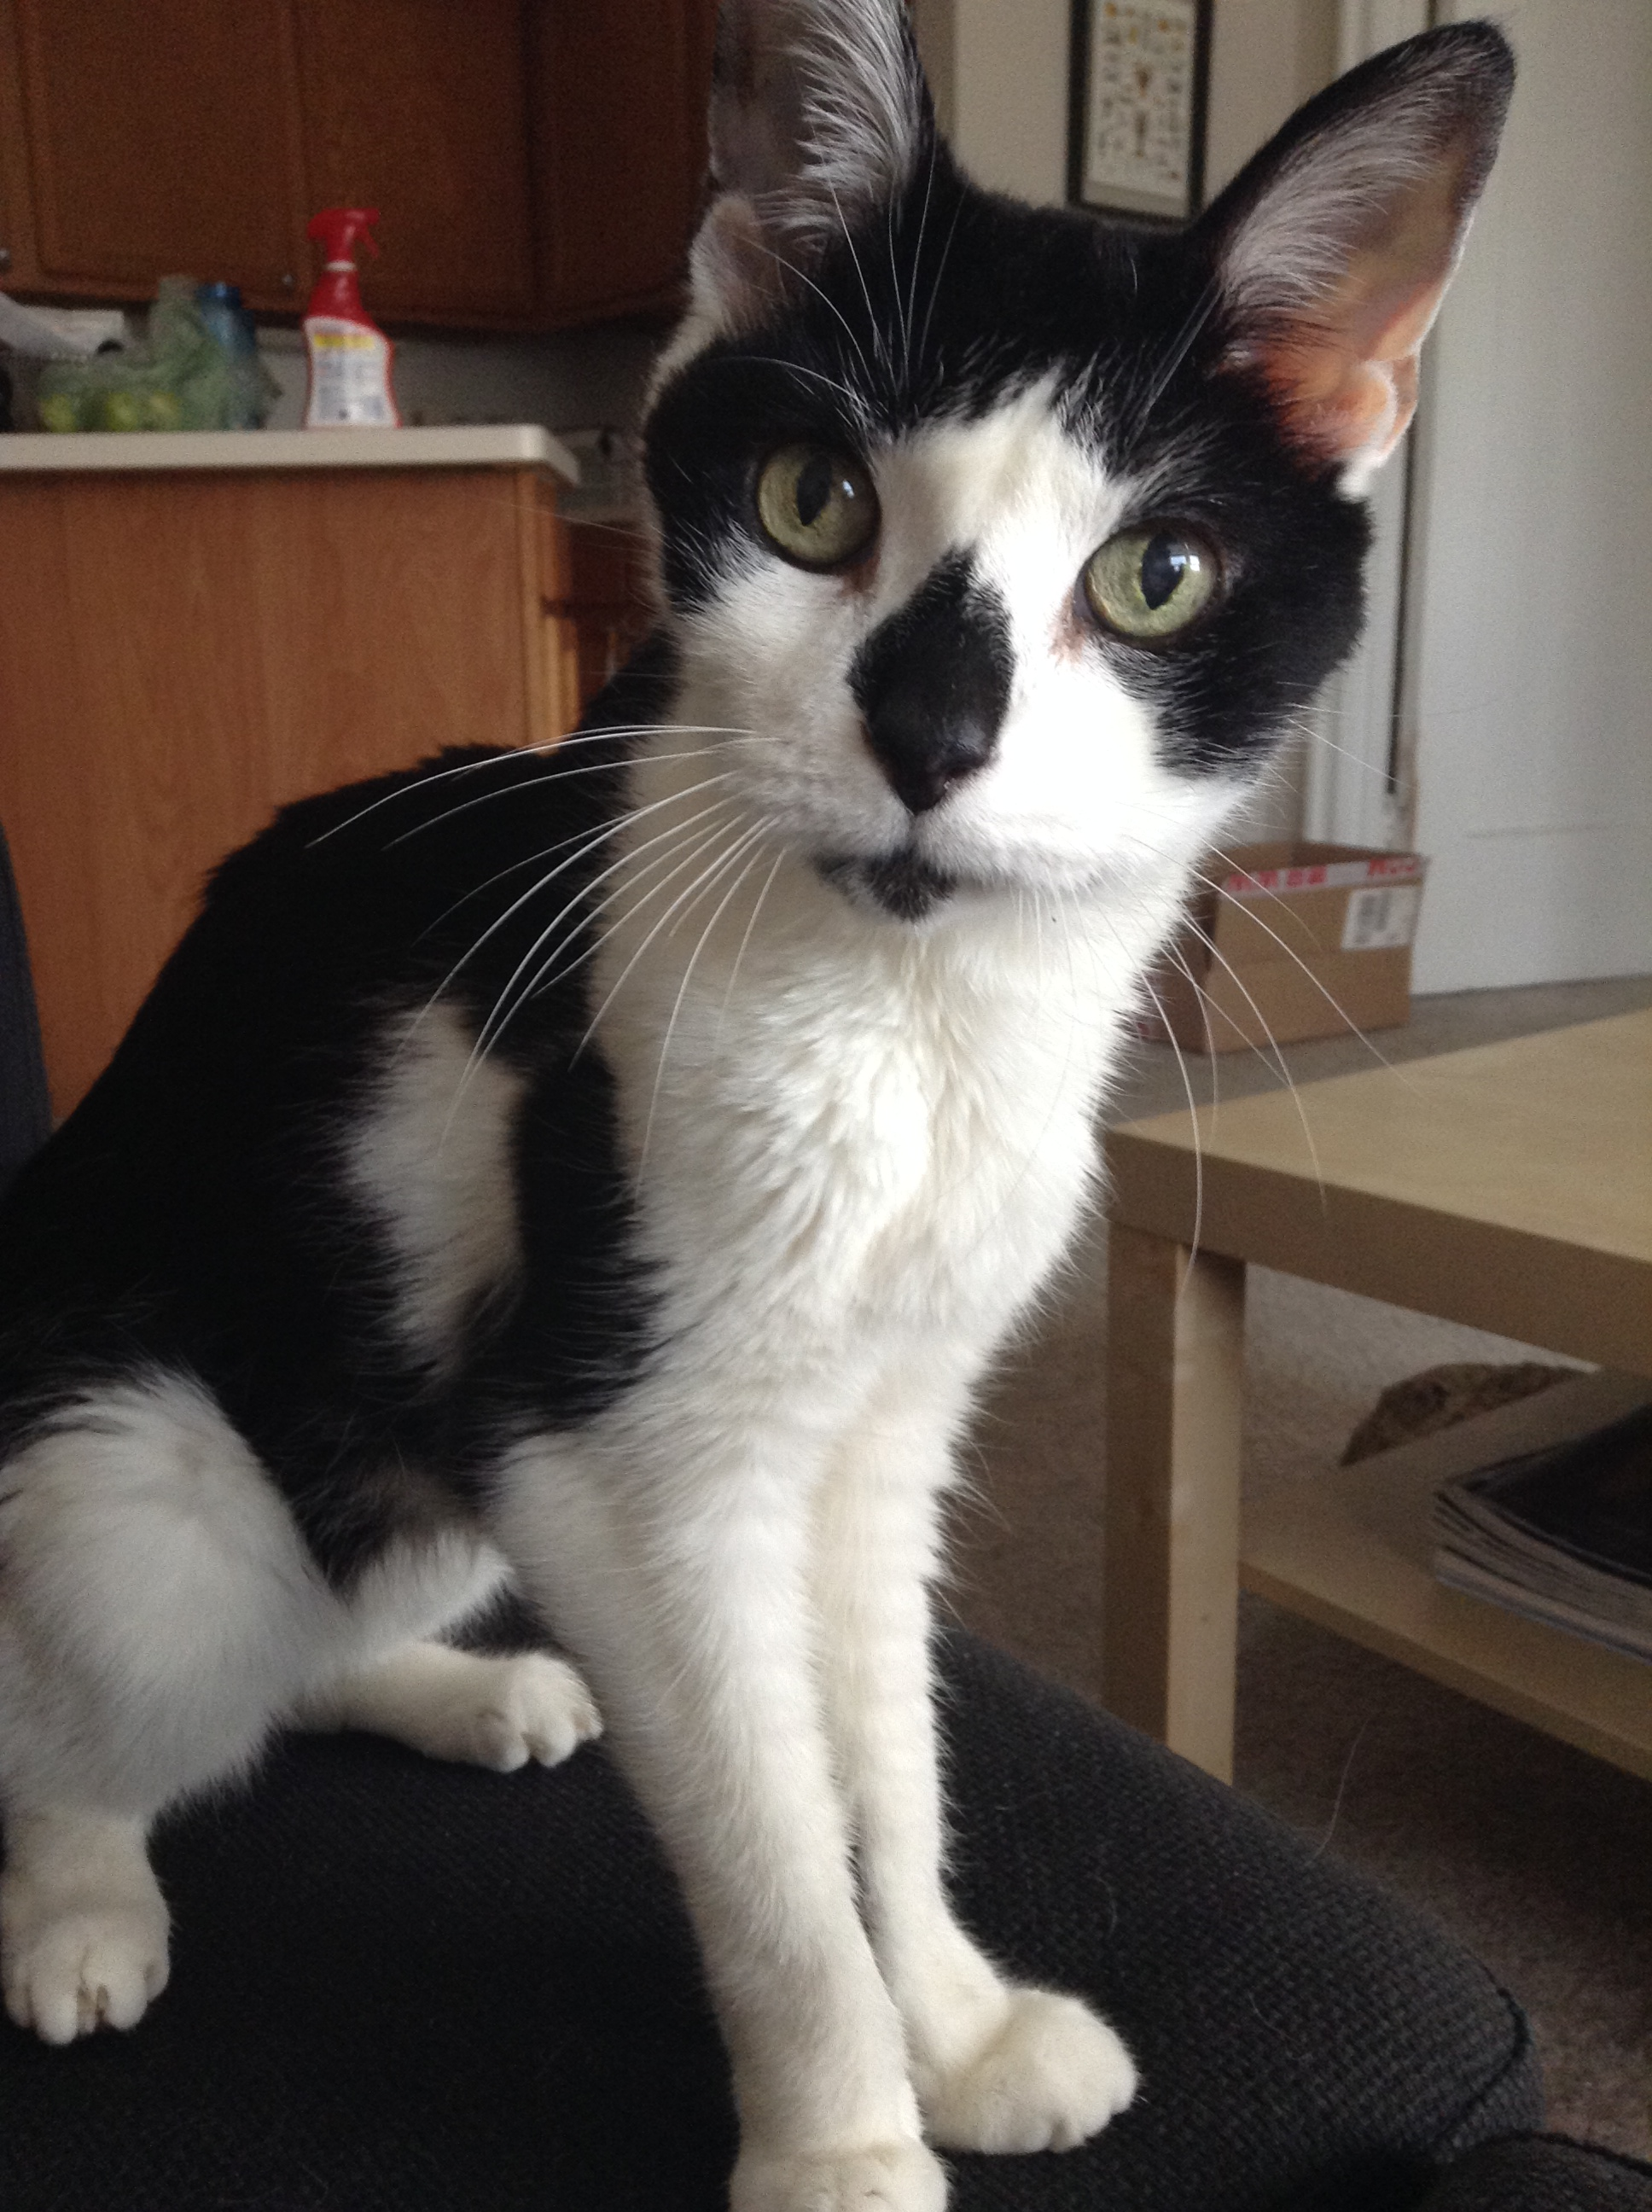
\includegraphics[height = 0.6\textheight, keepaspectratio = true]{figure/monty}
      \end{center}
    \end{column}
    \begin{column}{0.5\textwidth}
      \begin{center}
        \textbf{Brachiopods}

        \vspace{0.5cm}

        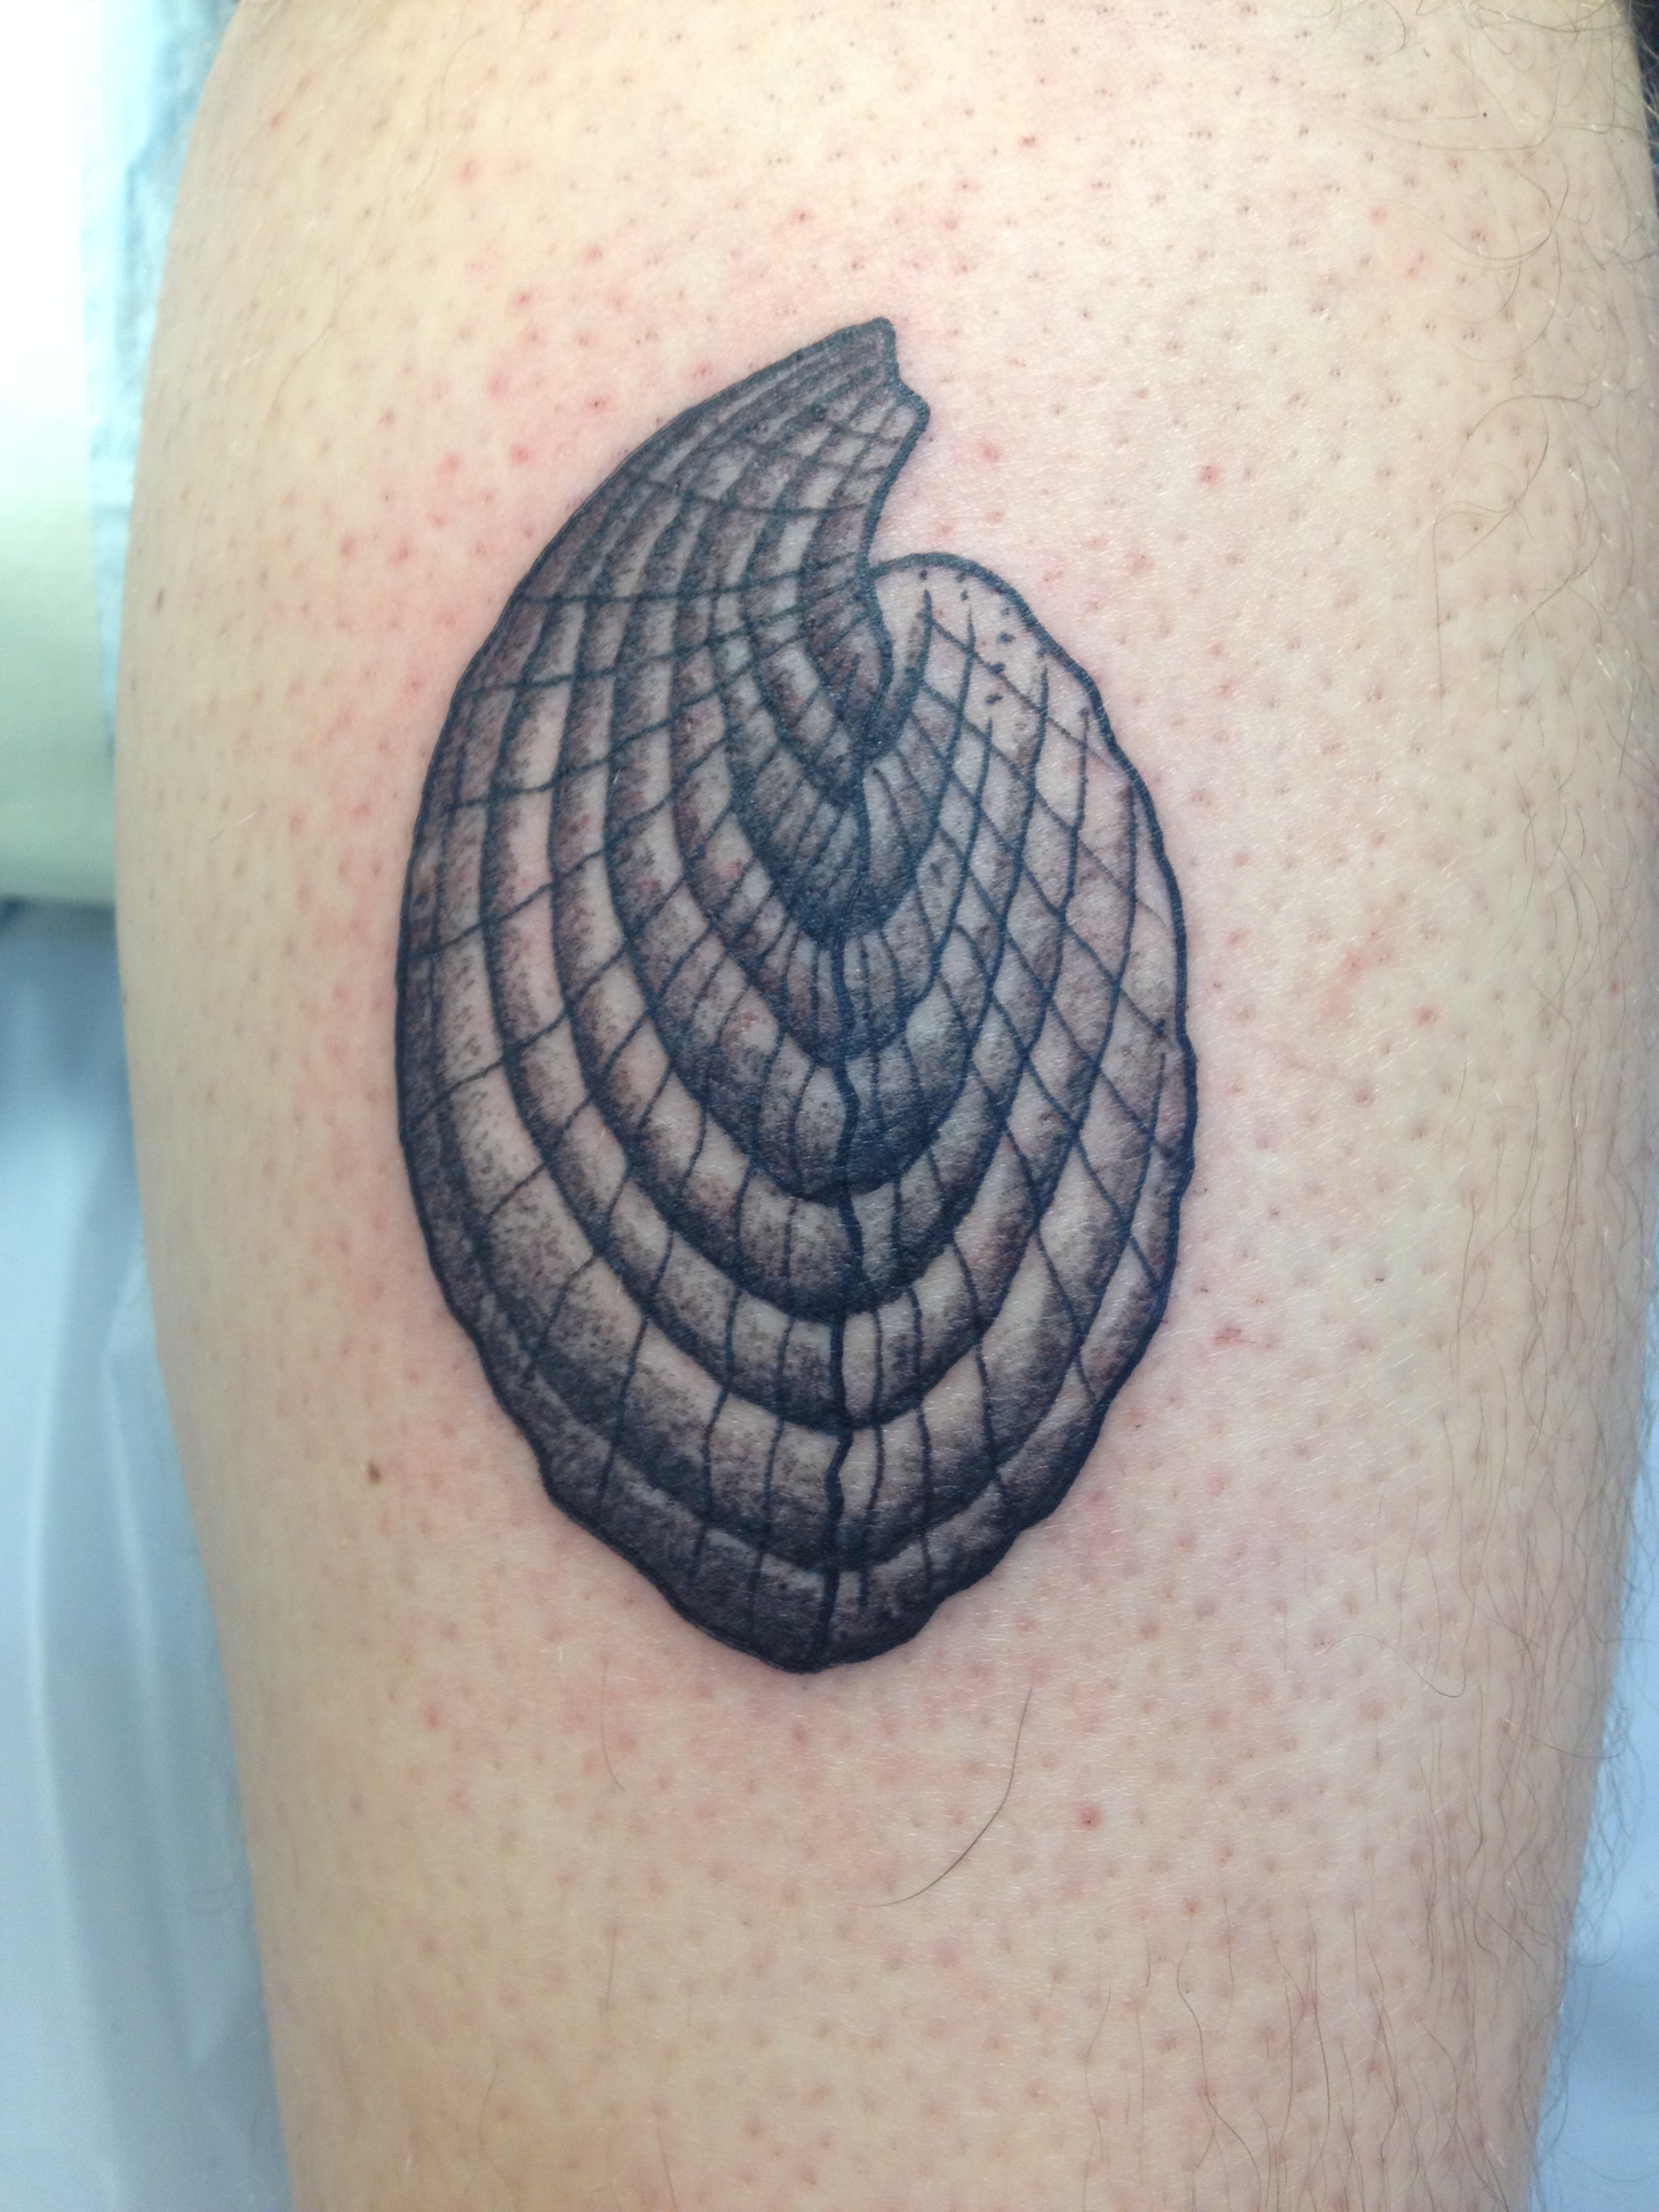
\includegraphics[height = 0.6\textheight, keepaspectratio = true]{figure/tattoo}
      \end{center}
    \end{column}
  \end{columns}
\end{frame}

\begingroup
\AtBeginSection{}
\section{Patterns in survival}
\endgroup
\subsection{Background extinction and expected differences in species survival}

\begin{frame}
  \frametitle{Age of Mammals}
  \begin{center}
    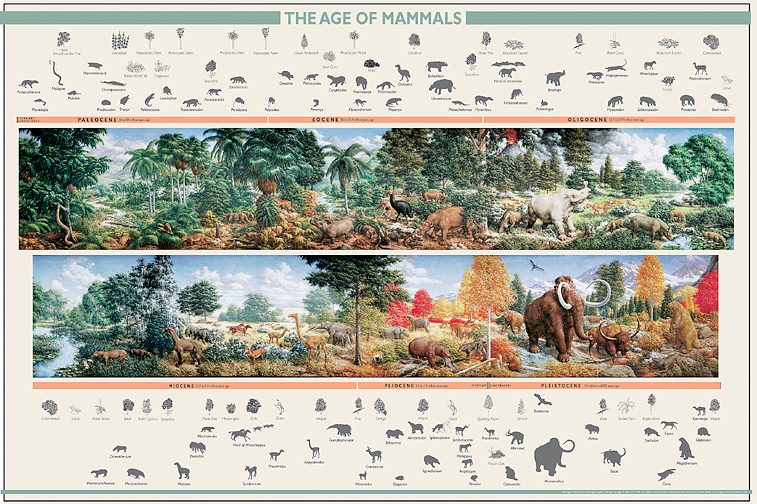
\includegraphics[width = \textwidth,height = 0.8\textheight,keepaspectratio = true]{figure/aom}
  \end{center}
\end{frame}

\begin{frame}
  \begin{alertblock}{Motivating questions}
    \begin{itemize}
      \item \alert{How do mammal species traits affect extinction risk?}
        \begin{itemize}
          \item How do shared time of origination or evolutionary history relate to extinction risk?
        \end{itemize}
      \item How do my findings compare to current risk factors?
      \item Is species extinction risk age-independent?
    \end{itemize}
  \end{alertblock}
\end{frame}

\begin{frame}
  \frametitle{Relationship between range size and extinction risk}
  \begin{center}
    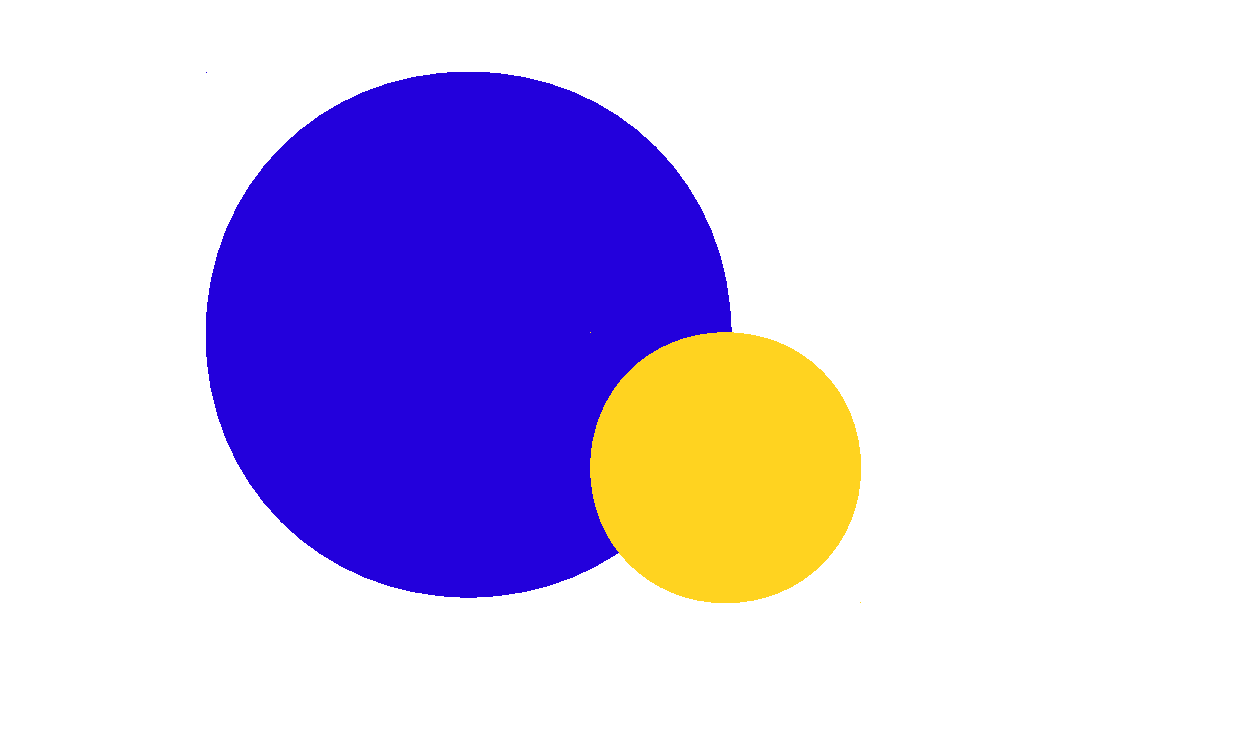
\includegraphics[width = \textwidth,height = 0.8\textheight,keepaspectratio = true]{figure/geo_range_1}
  \end{center}
\end{frame}

\begin{frame}
  \frametitle{Relationship between range size and extinction risk}
  \begin{center}
    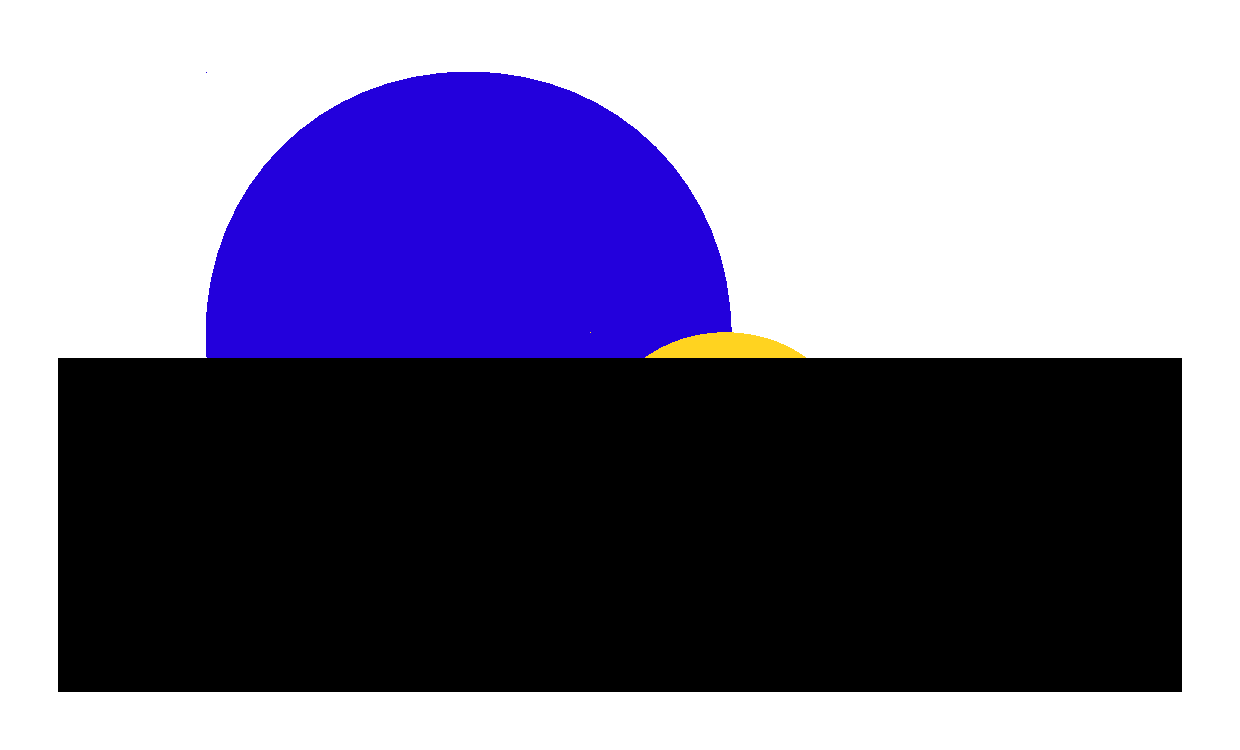
\includegraphics[width = \textwidth,height = 0.8\textheight,keepaspectratio = true]{figure/geo_range_2}
  \end{center}
\end{frame}

\begin{frame}
  \frametitle{Hypotheses of effects of locomotor category}
  \begin{center}
    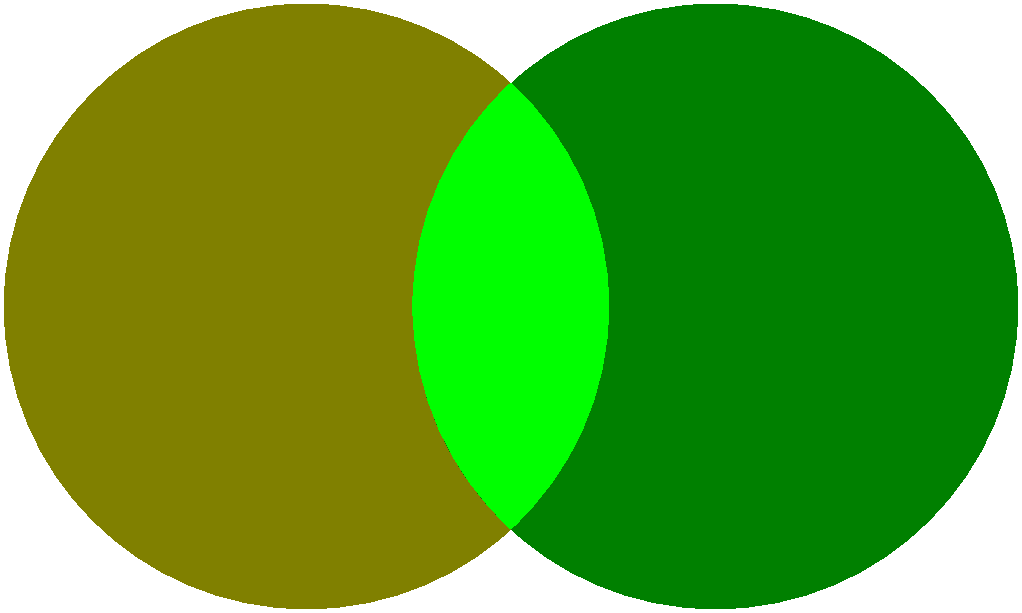
\includegraphics[width = \textwidth,height = 0.8\textheight,keepaspectratio = true]{figure/loco_initial}
  \end{center}
\end{frame}

\begin{frame}
  \frametitle{Hypotheses of effects of locomotor category}
  \begin{center}
    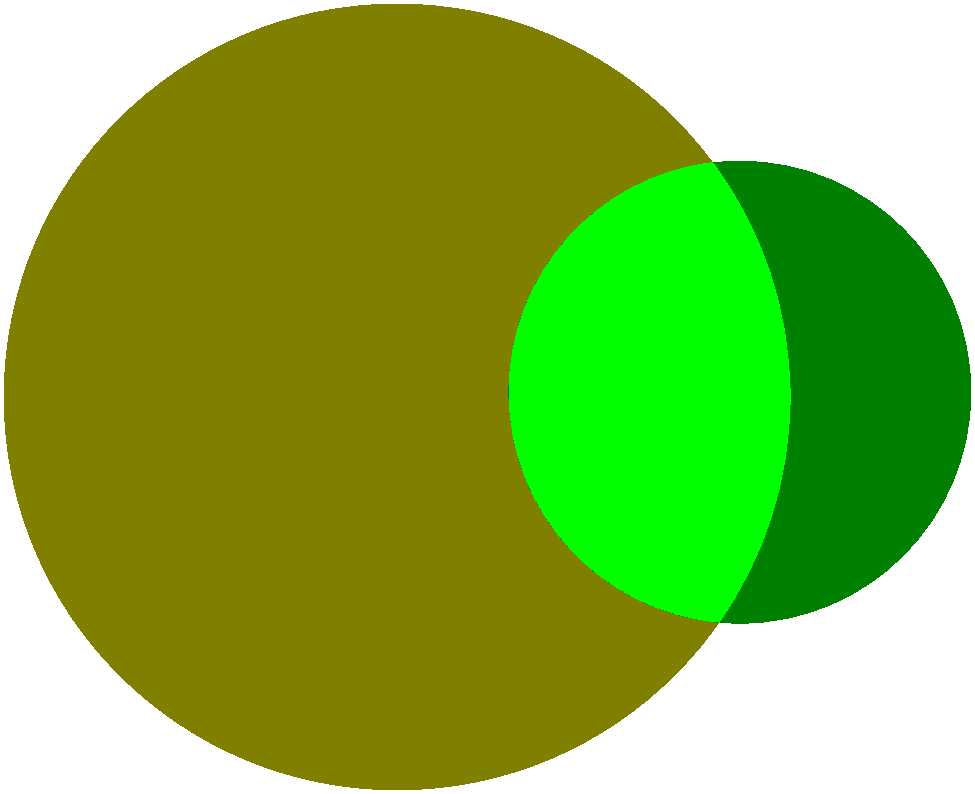
\includegraphics[width = \textwidth,height = 0.8\textheight,keepaspectratio = true]{figure/loco_later}
  \end{center}
\end{frame}

\begin{frame}
  \frametitle{Hypotheses of effects of dietary category}
  \begin{center}
    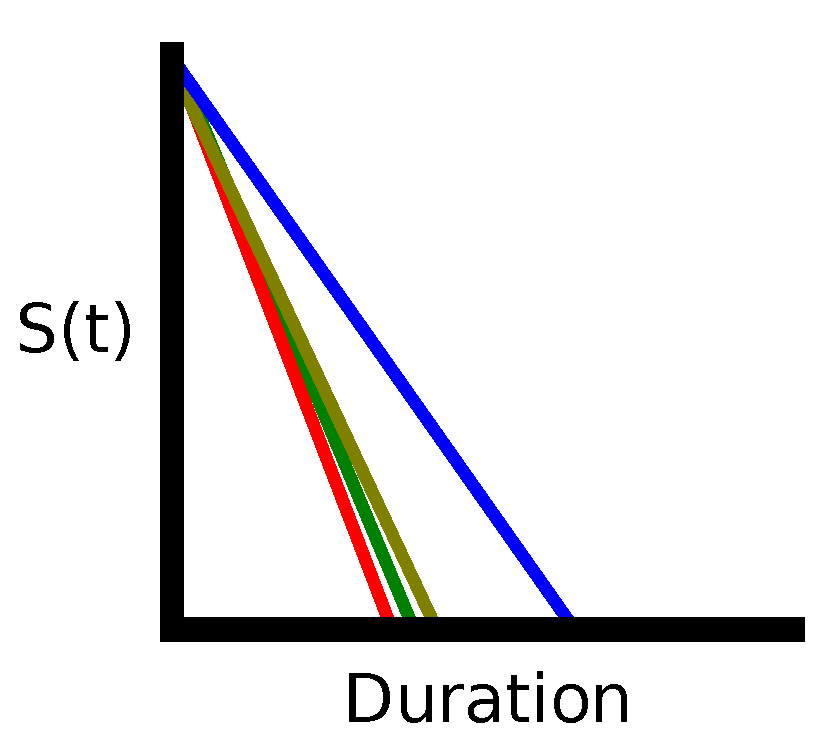
\includegraphics[width = \textwidth,height = 0.8\textheight,keepaspectratio = true]{figure/diet_survival}
  \end{center}
\end{frame}

\begin{frame}
  \frametitle{Survival model diagram}
  \begin{center}
    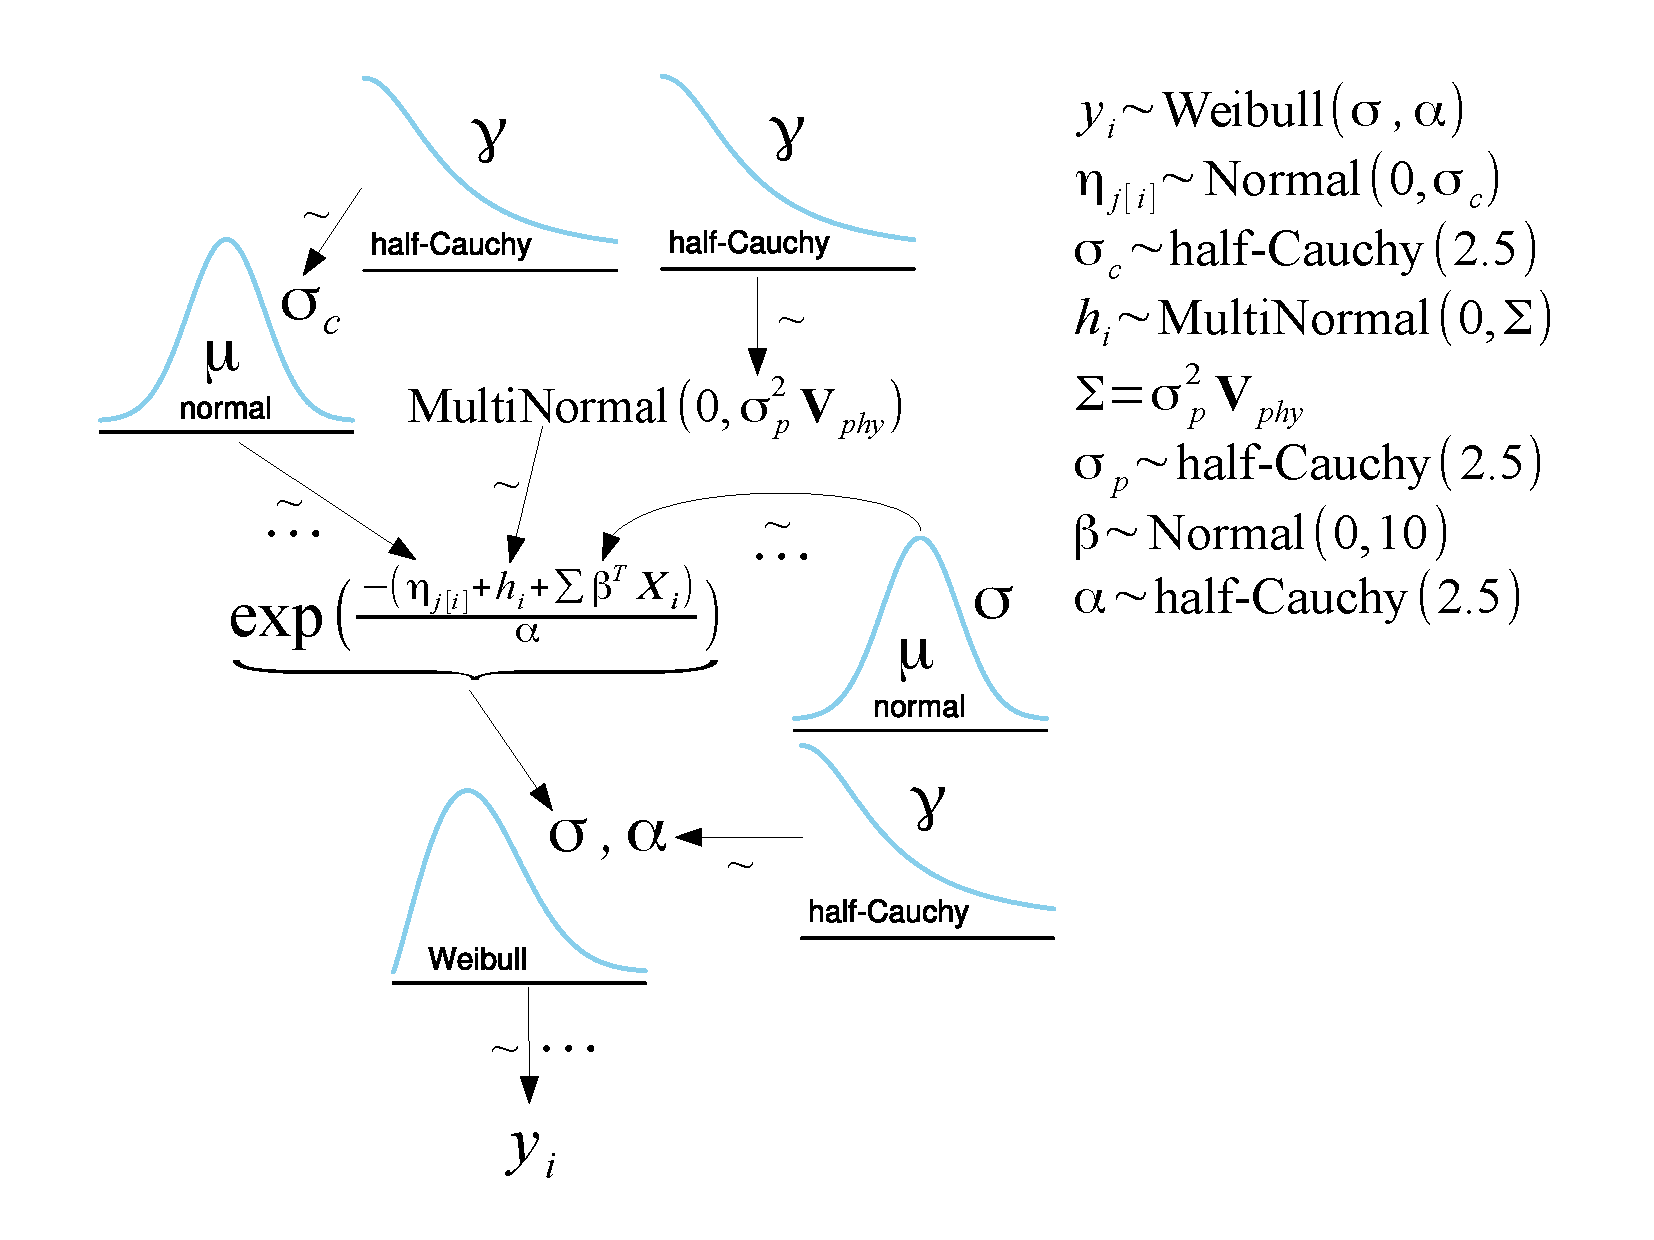
\includegraphics[height=0.8\textheight,keepaspectratio=true]{figure/mammal_survival_model}
  \end{center}
\end{frame}

\begin{frame}
  \frametitle{Pattern of species survival under two models}

  \begin{center}
    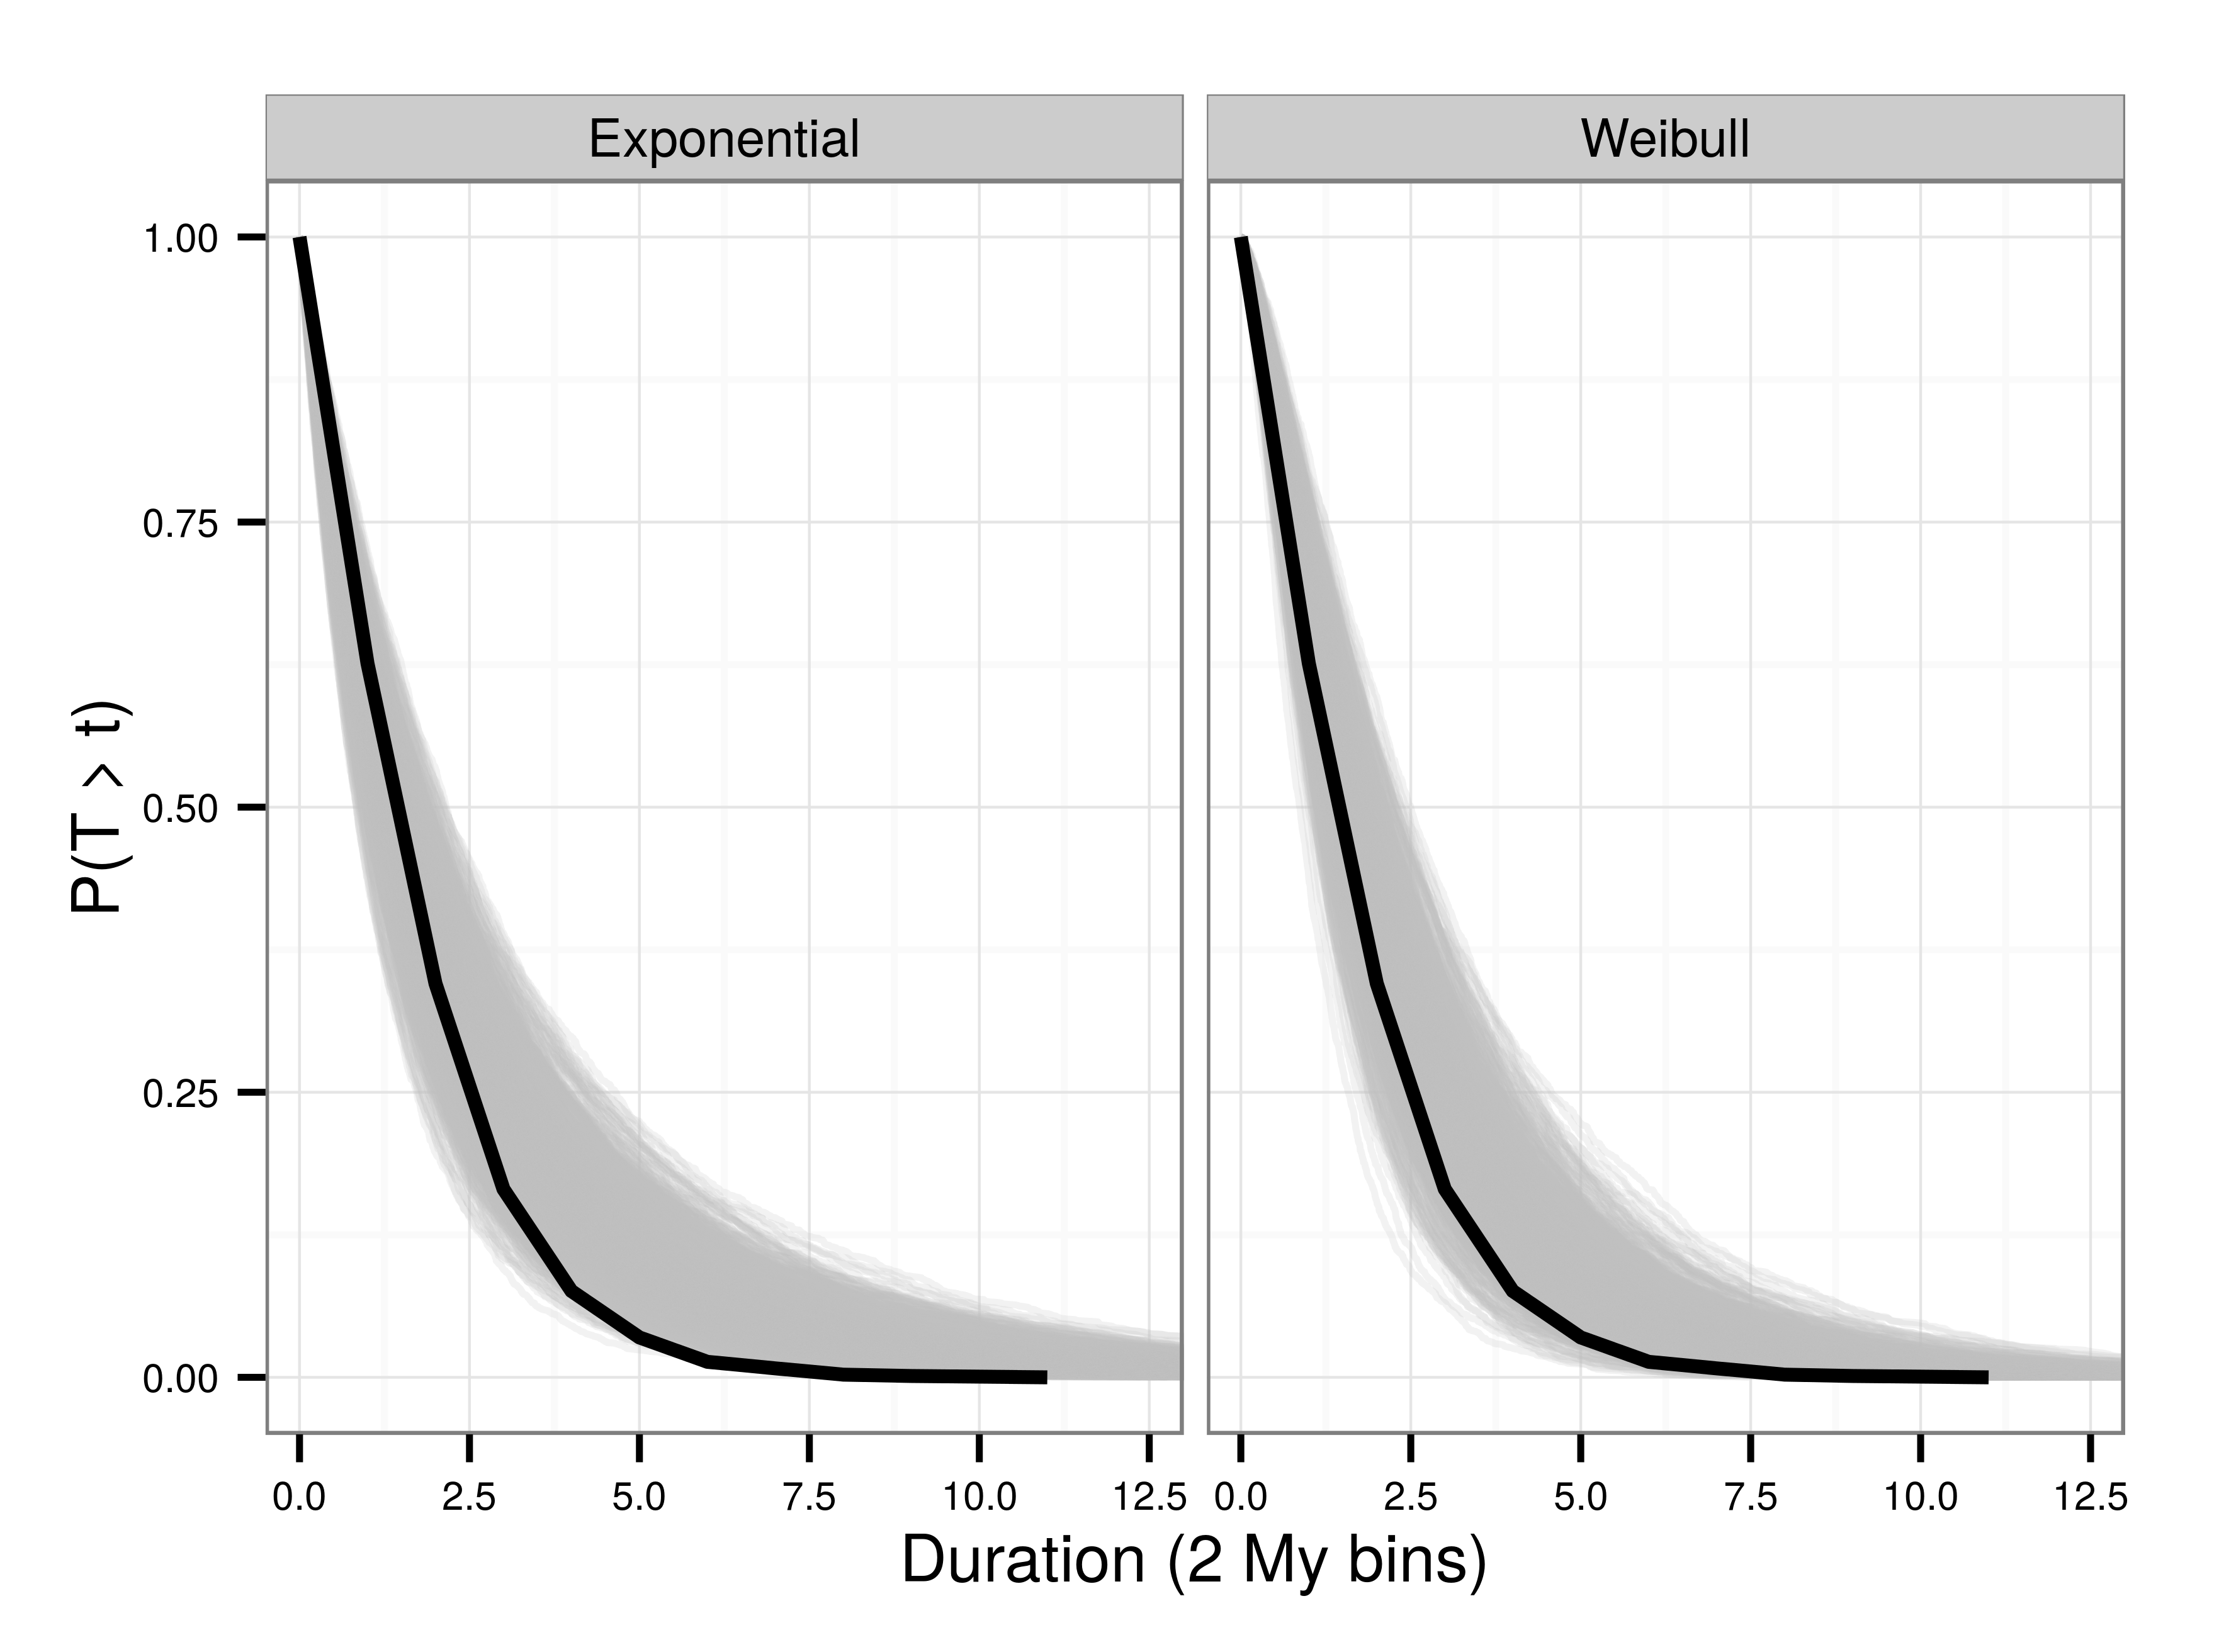
\includegraphics[height=0.75\textheight,keepaspectratio=true]{figure/survival_function_pres}
  \end{center}

  \tiny{\attrib{Smits 2015 \em{PNAS}}}
\end{frame}

\begin{frame}
  \frametitle{Effect of locomotor category on extinction risk}

  \begin{center}
    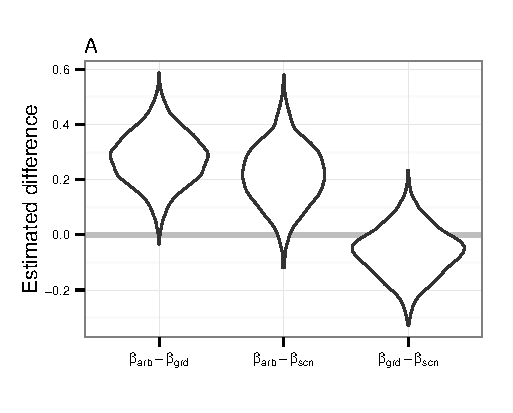
\includegraphics[height=0.75\textheight,keepaspectratio=true]{figure/loco_diff_est}
  \end{center}

  \tiny{\attrib{Smits 2015 \em{PNAS}}}
\end{frame}

\begin{frame}
  \frametitle{Effect of dietary category on extinction risk}

  \begin{center}
    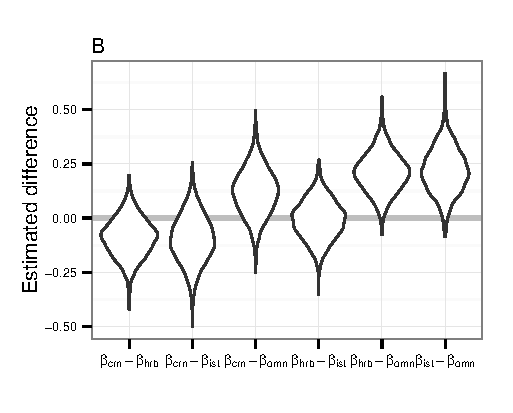
\includegraphics[height=0.8\textheight,keepaspectratio=true]{figure/diet_diff_est}
  \end{center}

  \tiny{\attrib{Smits 2015 \em{PNAS}}}
\end{frame}

\begin{frame}
  \frametitle{Difference in risk between origination cohorts}

  \begin{center}
    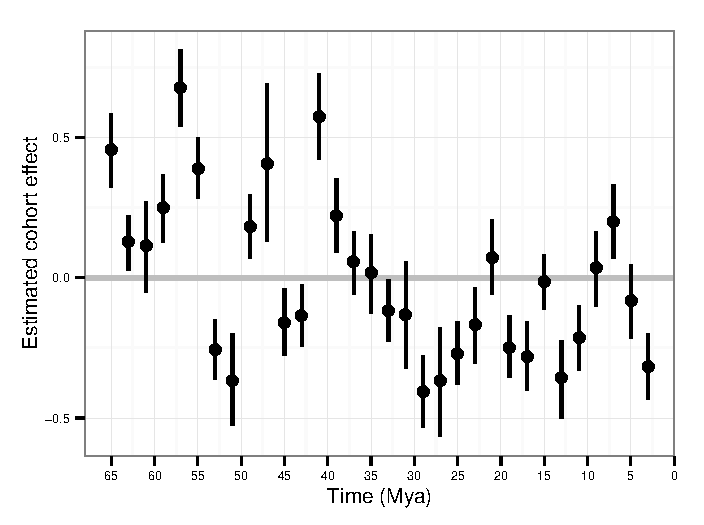
\includegraphics[height=0.8\textheight,keepaspectratio=true]{figure/cohort_est_pres}
  \end{center}

  \tiny{\attrib{Smits 2015 \em{PNAS}}}
\end{frame}

\begin{frame}
  \frametitle{Three sources of variance}

  \begin{center}
    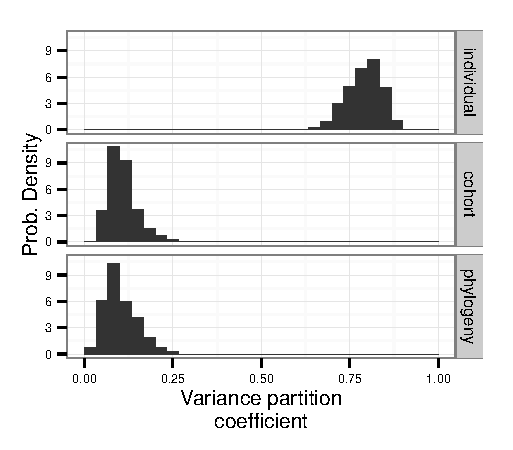
\includegraphics[height=0.8\textheight,keepaspectratio=true]{figure/variance_est}
  \end{center}

  \tiny{\attrib{Smits 2015 \em{PNAS}}}
\end{frame}

\begin{frame}
  \begin{block}{Summary of results}
    \begin{itemize}
      \item Survival of the unspecialized as time-invariant generalization.
      \item Decrease in extinction risk with time.
        \begin{itemize}
          \item Both cohort/temporal and phylogenetic effect.
        \end{itemize}
      \item Some incongruence with risk factors in the Recent.
        \begin{itemize}
          \item e.g. effect of body size, trophic category, phylogenetic clustering.
        \end{itemize}
    \end{itemize}
  \end{block}
\end{frame}



\subsection{Interplay between extinction intensity and extinction selectivity}

\begin{frame}
  \begin{alertblock}{Jablonski 1986 \em{Science}}
    At K/Pg mass extinction, biological traits (except geographic range) have no effect on \alert{bivalve} taxonomic survival.
  \end{alertblock}

\end{frame}


\begin{frame}
  \frametitle{Variation in extinction rate}
  \begin{center}
    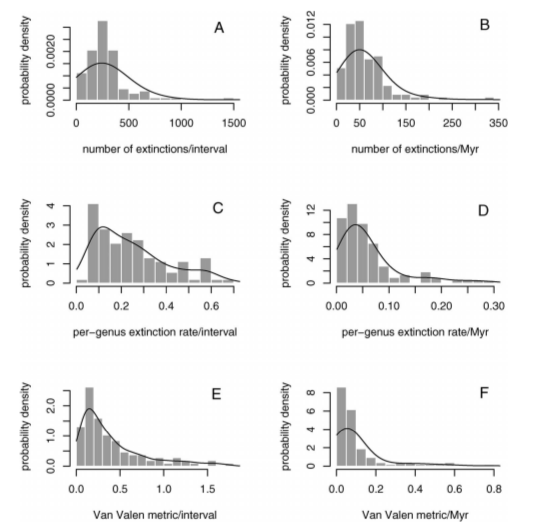
\includegraphics[width = \textwidth,height = 0.8\textheight,keepaspectratio = true]{figure/wang_extinction}
  \end{center}

  \tiny{\attrib{Wang 2003 \em{Paleobio.}}}
\end{frame}

\begin{frame}
  \frametitle{Intensity and selectivity}
  \begin{center}
    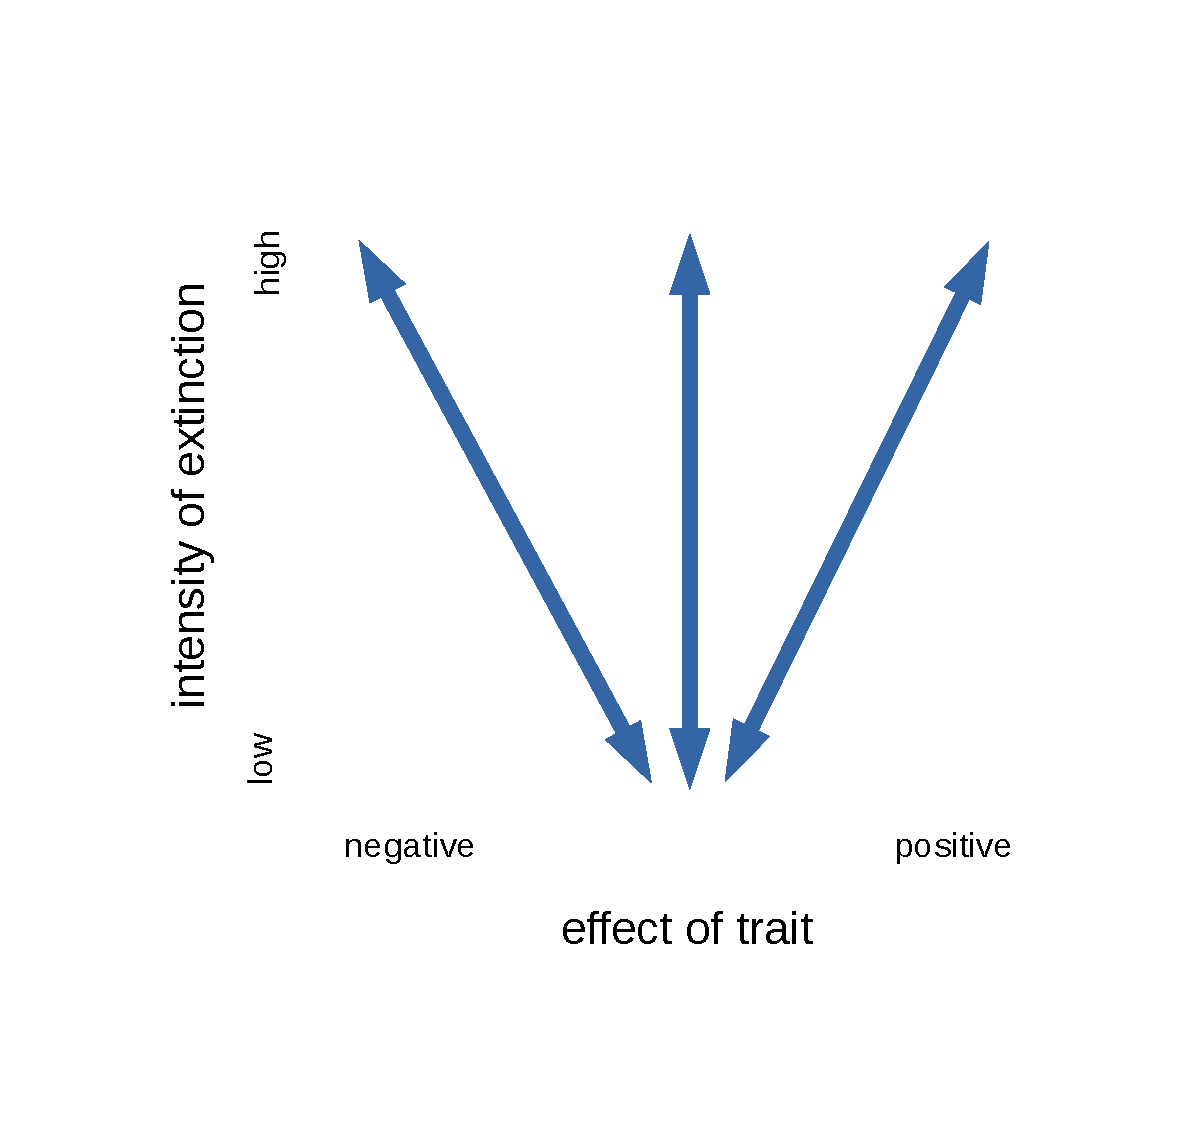
\includegraphics[width = \textwidth,height = 0.8\textheight,keepaspectratio = true]{figure/intensity_selectivity_base}
  \end{center}
\end{frame}

\begin{frame}
  \begin{alertblock}{Questions and analysis}
    How do the effect of traits on duration (\alert{extinction selectivity}) vary with expected duration (\alert{extinction intensity})?
  \end{alertblock}
\end{frame}

\begin{frame}
  \frametitle{Brachiopods}
  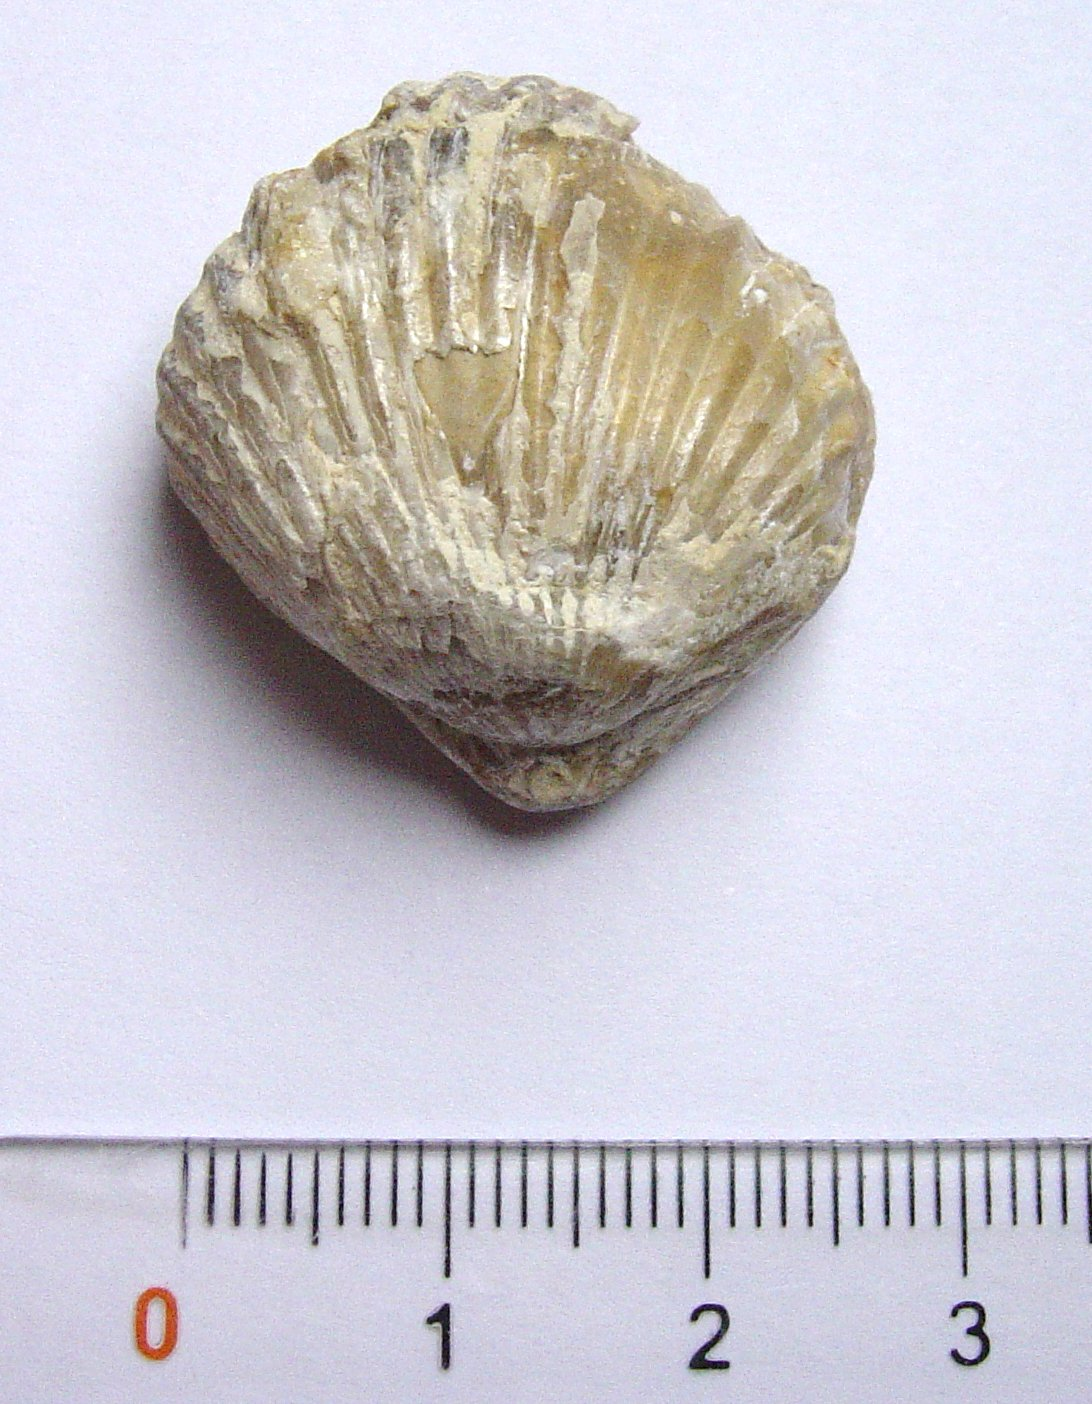
\includegraphics[width = 0.45\textwidth,height = 0.8\textheight,keepaspectratio = true]{figure/Brachiopod_fossil}
  \includegraphics[width = 0.45\textwidth,height = 0.8\textheight,keepaspectratio = true]{figure/Burmirhynchionella_decorata_brachial_CRF}

  \tiny{\attrib{ComputerHotline wikimedia CC BY 2.5; Dwergenpaartje wikimedia CC BY-SA 3.0}}
\end{frame}

\begin{frame}
  \frametitle{Post-Cambrian Paleozoic brachiopod genera and covariates}
  \begin{itemize}
    \item time range approx. 488-252 Mya.
    \item stage as time unit; duration measured in stages (2-5 My each)
    \item effect of traits varies by origination cohort
      \begin{itemize}
        \item geographic range
        \item body size
        \item environmental preference (v, v\(^2\))
      \end{itemize}
    \item gap statistic as measure of sampling (Foote and Raup 1996 \em{Paleobio}), imputed for taxa with short durations
  \end{itemize}
\end{frame}

\begin{frame}
  \frametitle{Hierarchical survival model}
  \begin{center}
    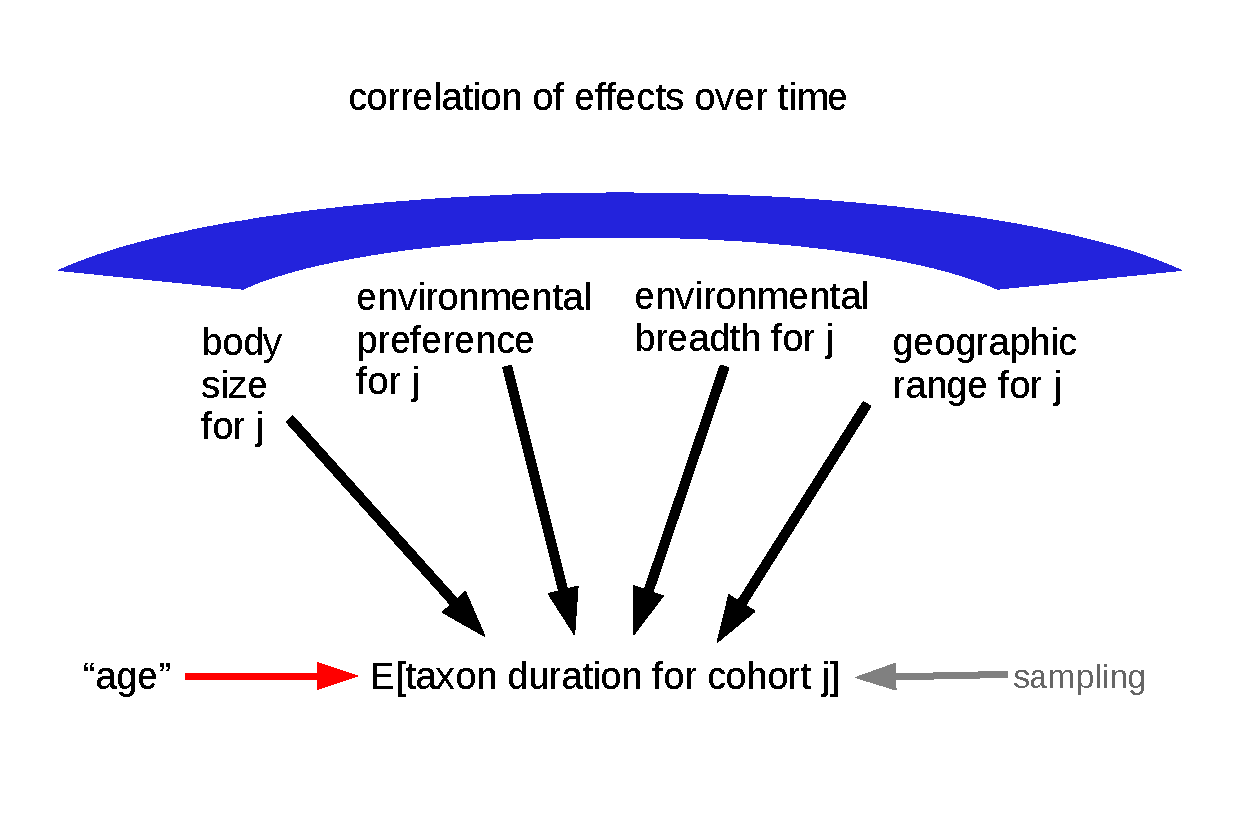
\includegraphics[width = \textwidth,height = 0.8\textheight,keepaspectratio = true]{figure/simple_model}
  \end{center}
\end{frame}

\begin{frame}
  \frametitle{Sampling statement for the joint posterior probability}
  \begin{columns}
    \begin{column}{0.5\textwidth}
      \begin{align*}
        y_{i, t} &\sim \text{Weibull}(\sigma_{i, t}, \alpha) \\
        \log(\sigma_{i, t}) &= \frac{X_{i}B_{j[i], t} + \delta s_{i}}{\alpha} \\
        B_{j} &\sim \text{MVN}(\mu, \Sigma) \\
        \Sigma &= \text{diag}(\tau) \Omega \text{diag}(\tau) \\
        s_{i} &\sim \text{Beta}(\phi_{i}, \lambda) \\
        \phi_{i} &= \text{logit}^{-1}(W_{i}\gamma) \\
      \end{align*}
    \end{column}
    \begin{column}{0.5\textwidth}
      \begin{align*}
        \mu_{intensity} &\sim \mathcal{N}(0, 5) \\
        \mu_{range} &\sim \mathcal{N}(-1, 1) \\
        \mu_{env pref} &\sim \mathcal{N}(0, 1) \\
        \mu_{env curve} &\sim \mathcal{N}(1, 1) \\
        \mu_{size} &\sim \mathcal{N}(0, 1) \\
        \delta &\sim \mathcal{N}(0, 1) \\
        \tau &\sim \text{C}^{+}(1) \\
        \Omega &\sim \text{LKJ}(1) \\
        \lambda &\sim \text{Pareto}(0.1, 1.5) \\
        \gamma &\sim \mathcal{N}(0, 1) \\
      \end{align*}
    \end{column}
  \end{columns}

  \scriptsize{Note: Calculation of log probability of right and left censored observations is modified from the above}
\end{frame}

%\begin{frame}
%  \frametitle{Model adequacy}
%  \begin{columns}
%    \begin{column}{0.5\textwidth}
%      \begin{center}
%        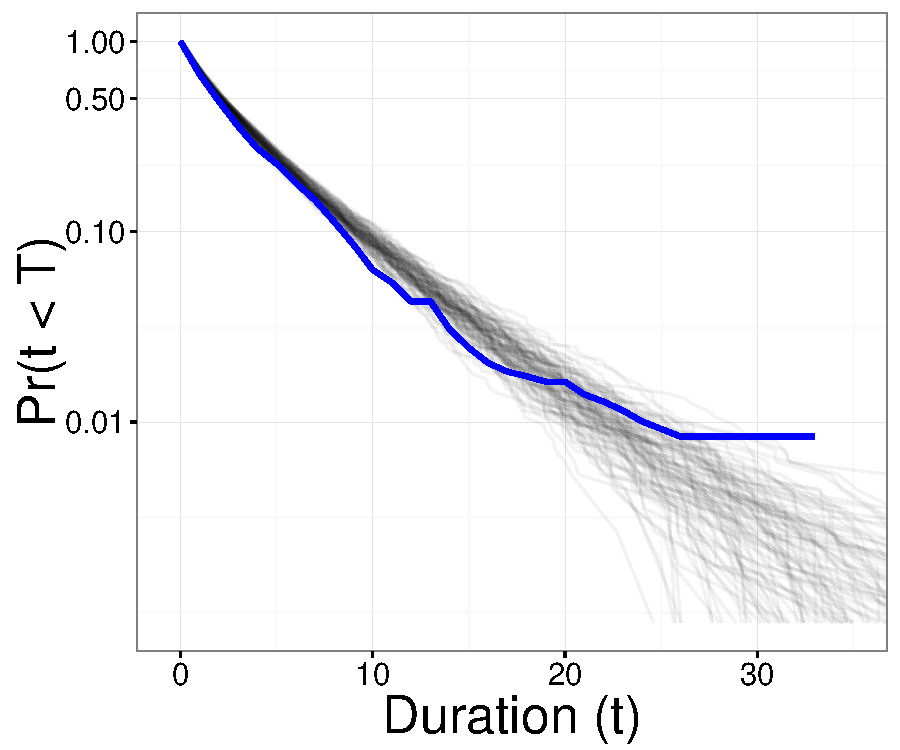
\includegraphics[width=\textwidth,height=0.8\textheight,keepaspectratio=true]{figure/survival_curves}
%      \end{center}
%    \end{column}
%    \begin{column}{0.5\textwidth}
%      \begin{center}
%        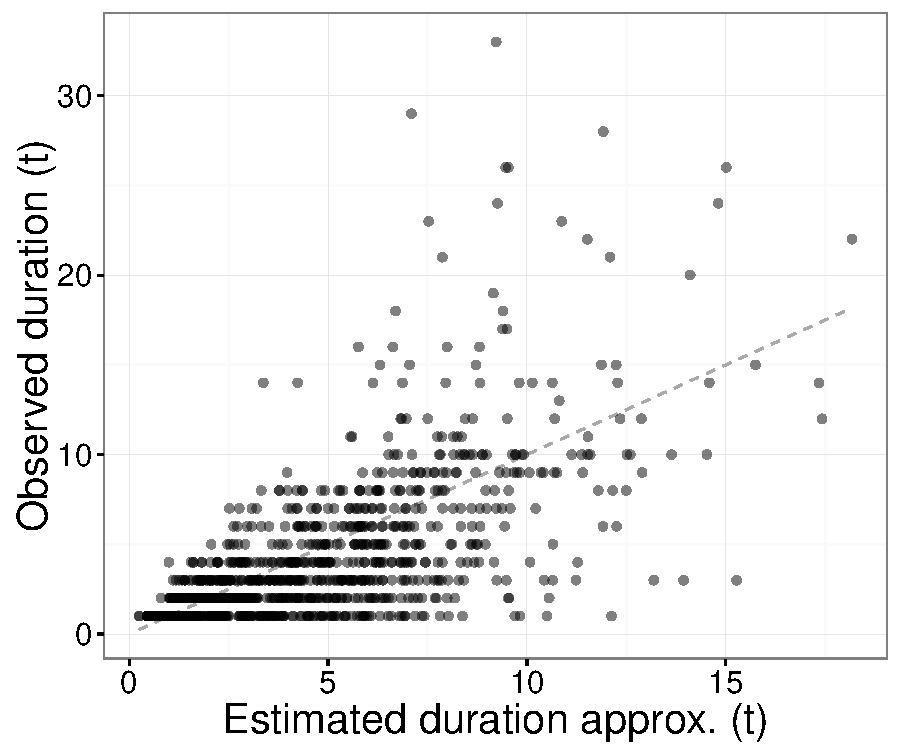
\includegraphics[width=\textwidth,height=0.8\textheight,keepaspectratio=true]{figure/shotgun}
%      \end{center}
%    \end{column}
%  \end{columns}
%\end{frame}

\begin{frame}
  \frametitle{Variation in trait effects between cohorts}

  \begin{center}
    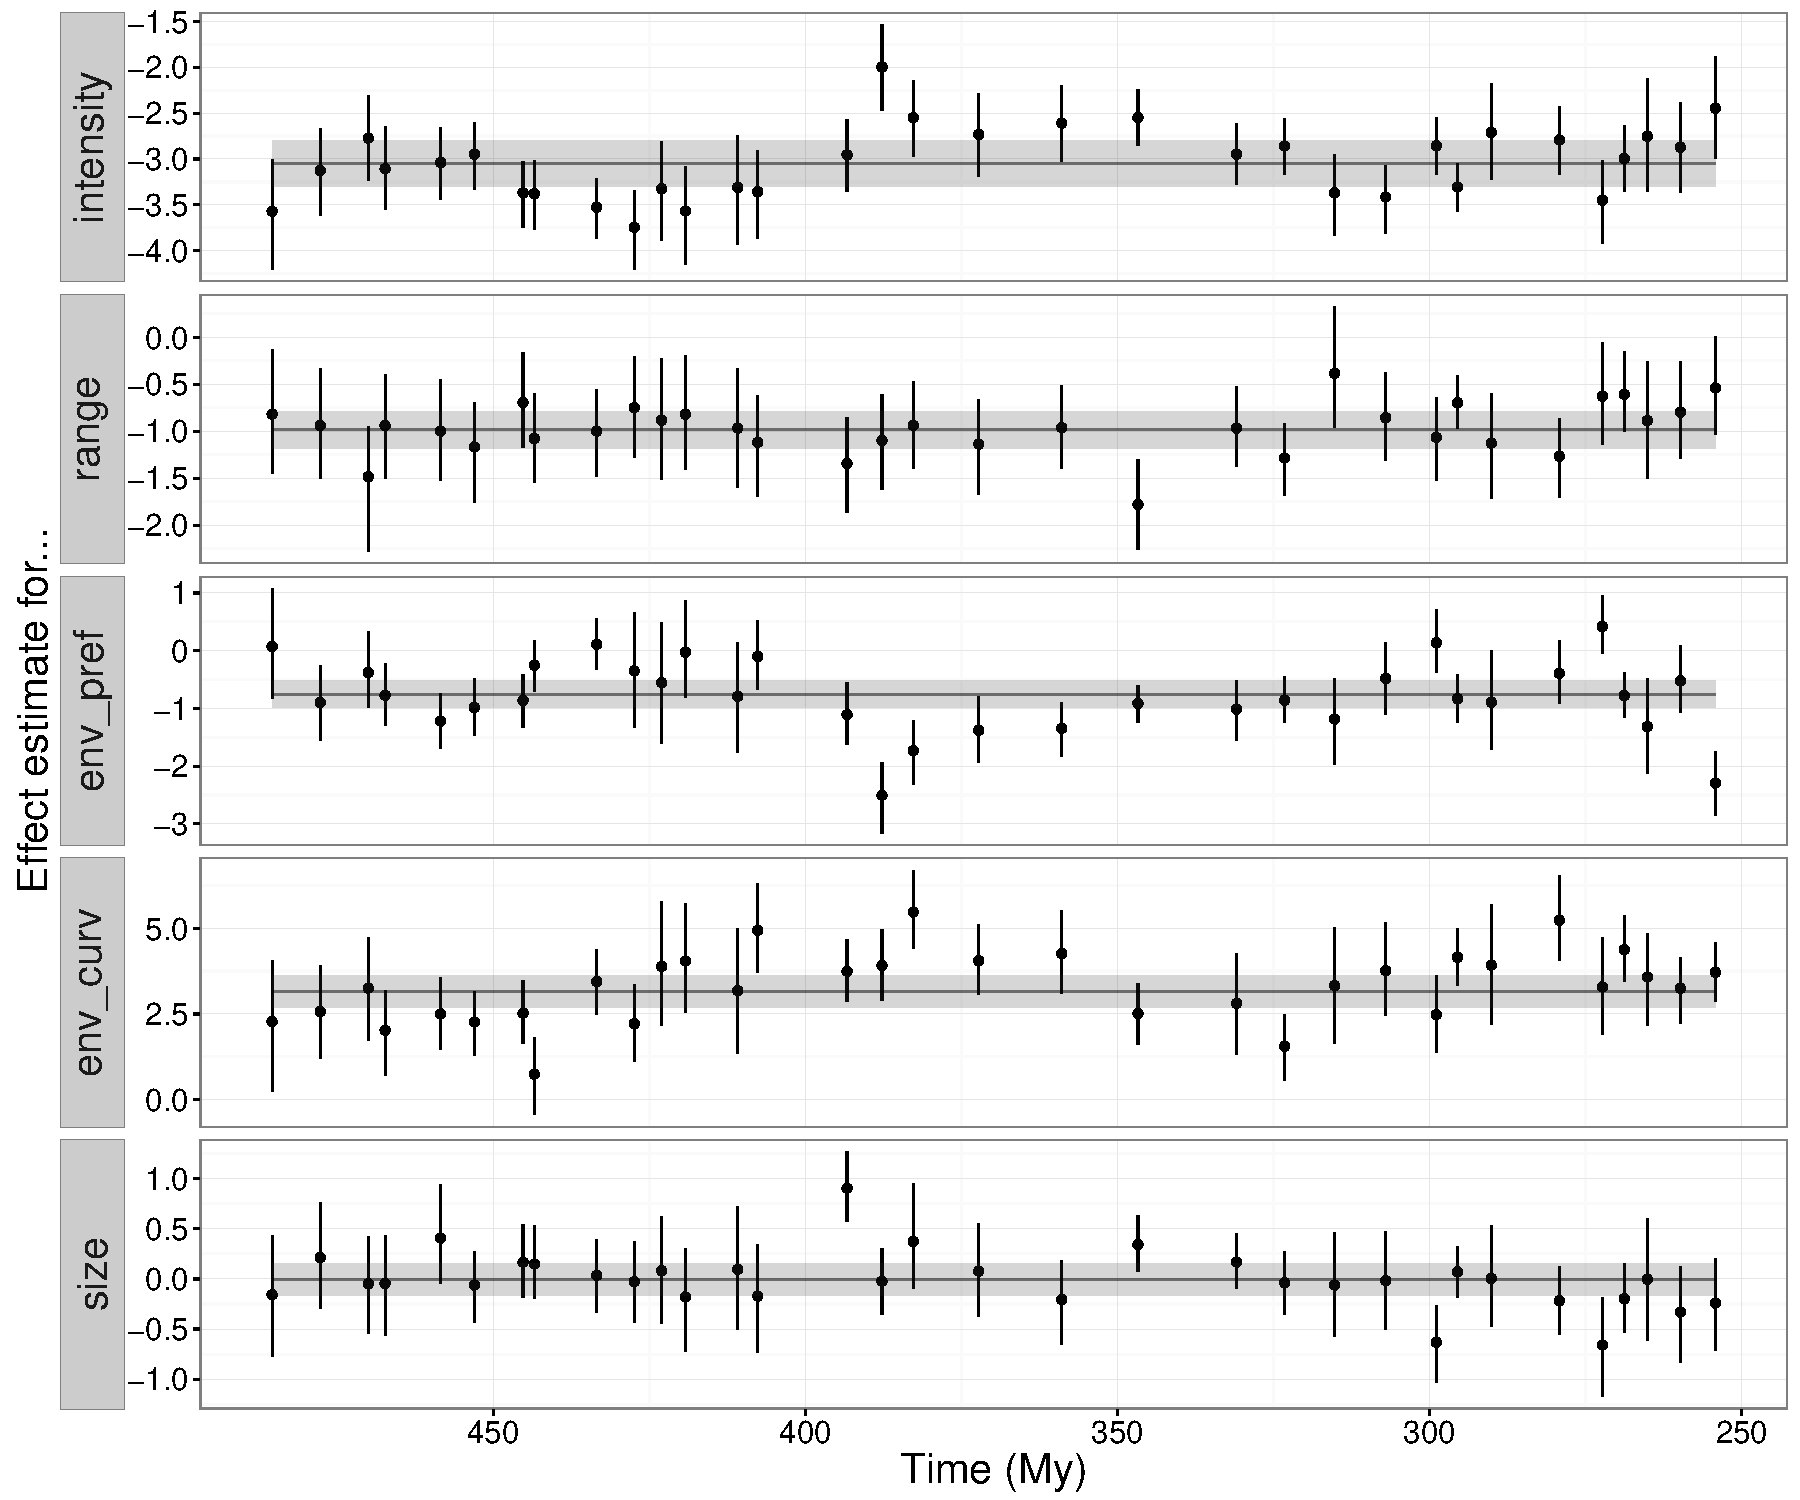
\includegraphics[width = \textwidth,height = 0.8\textheight,keepaspectratio = true]{figure/cohort_series_wide}
  \end{center}
\end{frame}

\begin{frame}
  \frametitle{Overall effect of environmental preference}

  \begin{center}
    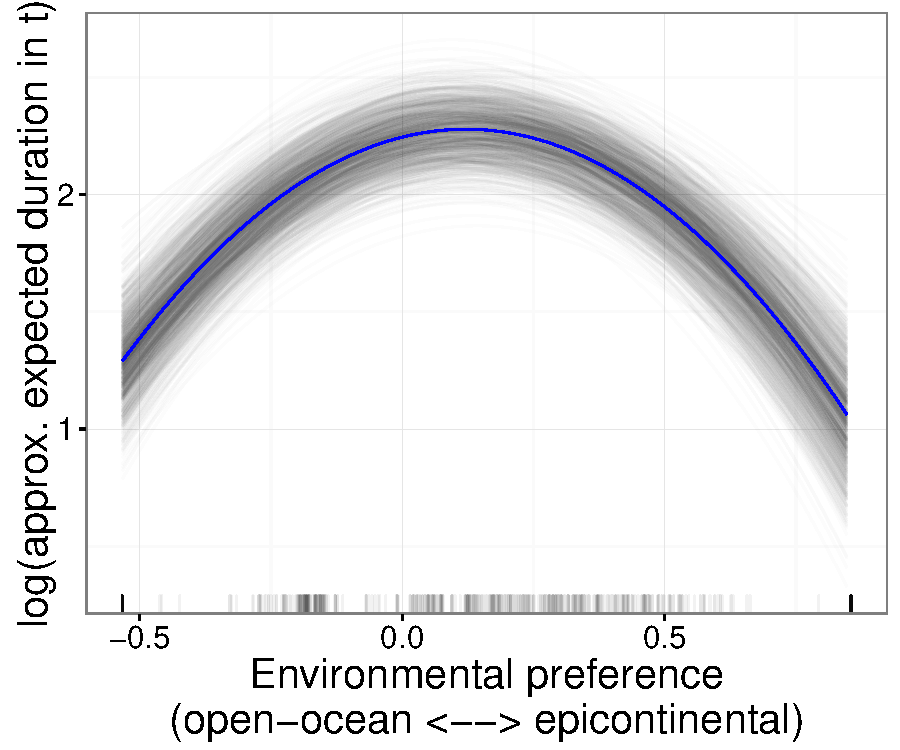
\includegraphics[width = \textwidth,height = 0.8\textheight,keepaspectratio = true]{figure/env_effect}
  \end{center}
\end{frame}

\begin{frame}
  \frametitle{Change in effect of environment between cohorts}

  \begin{center}
    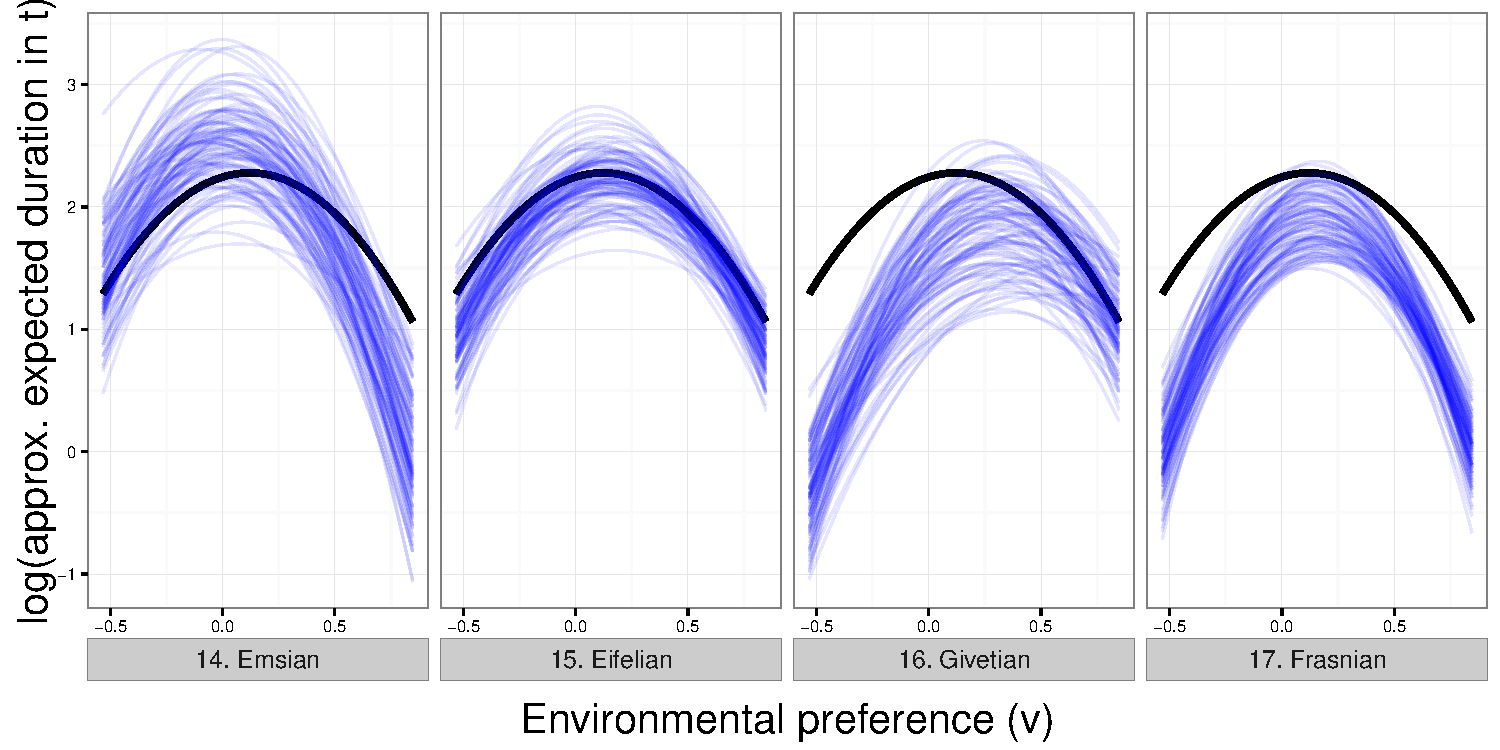
\includegraphics[width = \textwidth,height = 0.8\textheight,keepaspectratio = true]{figure/env_cohort_short}
  \end{center}
\end{frame}

\begin{frame}
  \frametitle{Change in effect of environment between cohorts}

  \begin{center}
    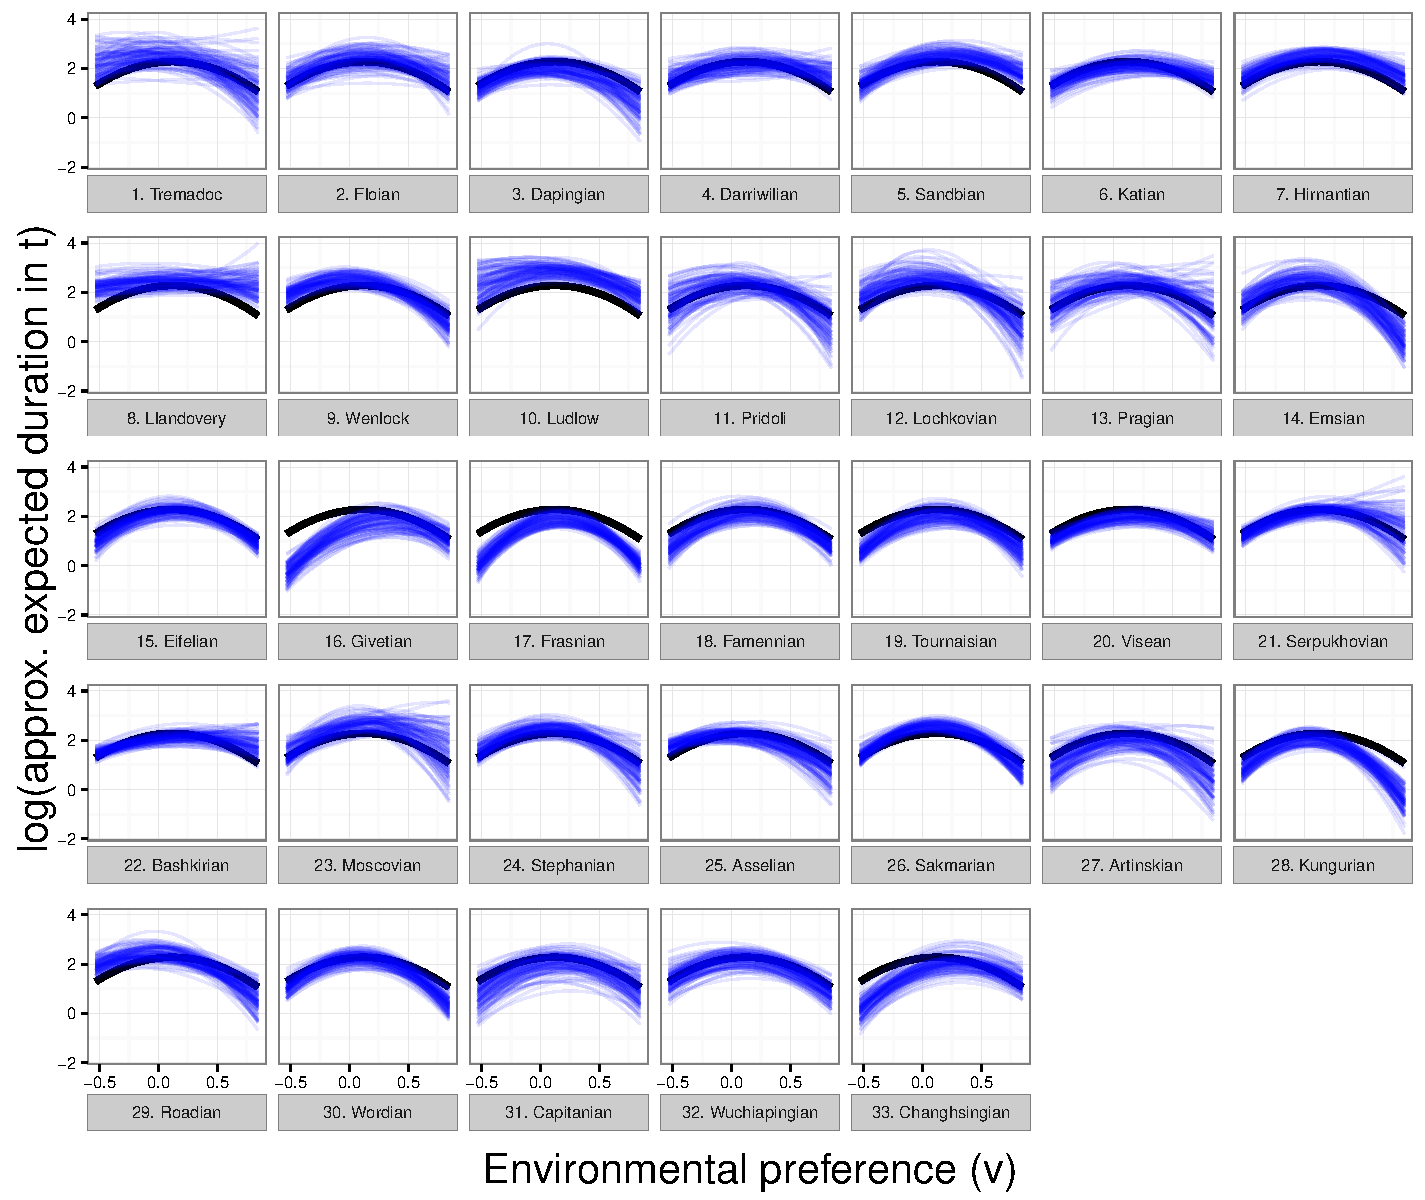
\includegraphics[width = 0.8\textwidth,height = 0.8\textheight,keepaspectratio = true]{figure/env_cohort_wide}
  \end{center}
\end{frame}

\begin{frame}
  \frametitle{Correlation of effects between cohorts}

  \begin{center}
    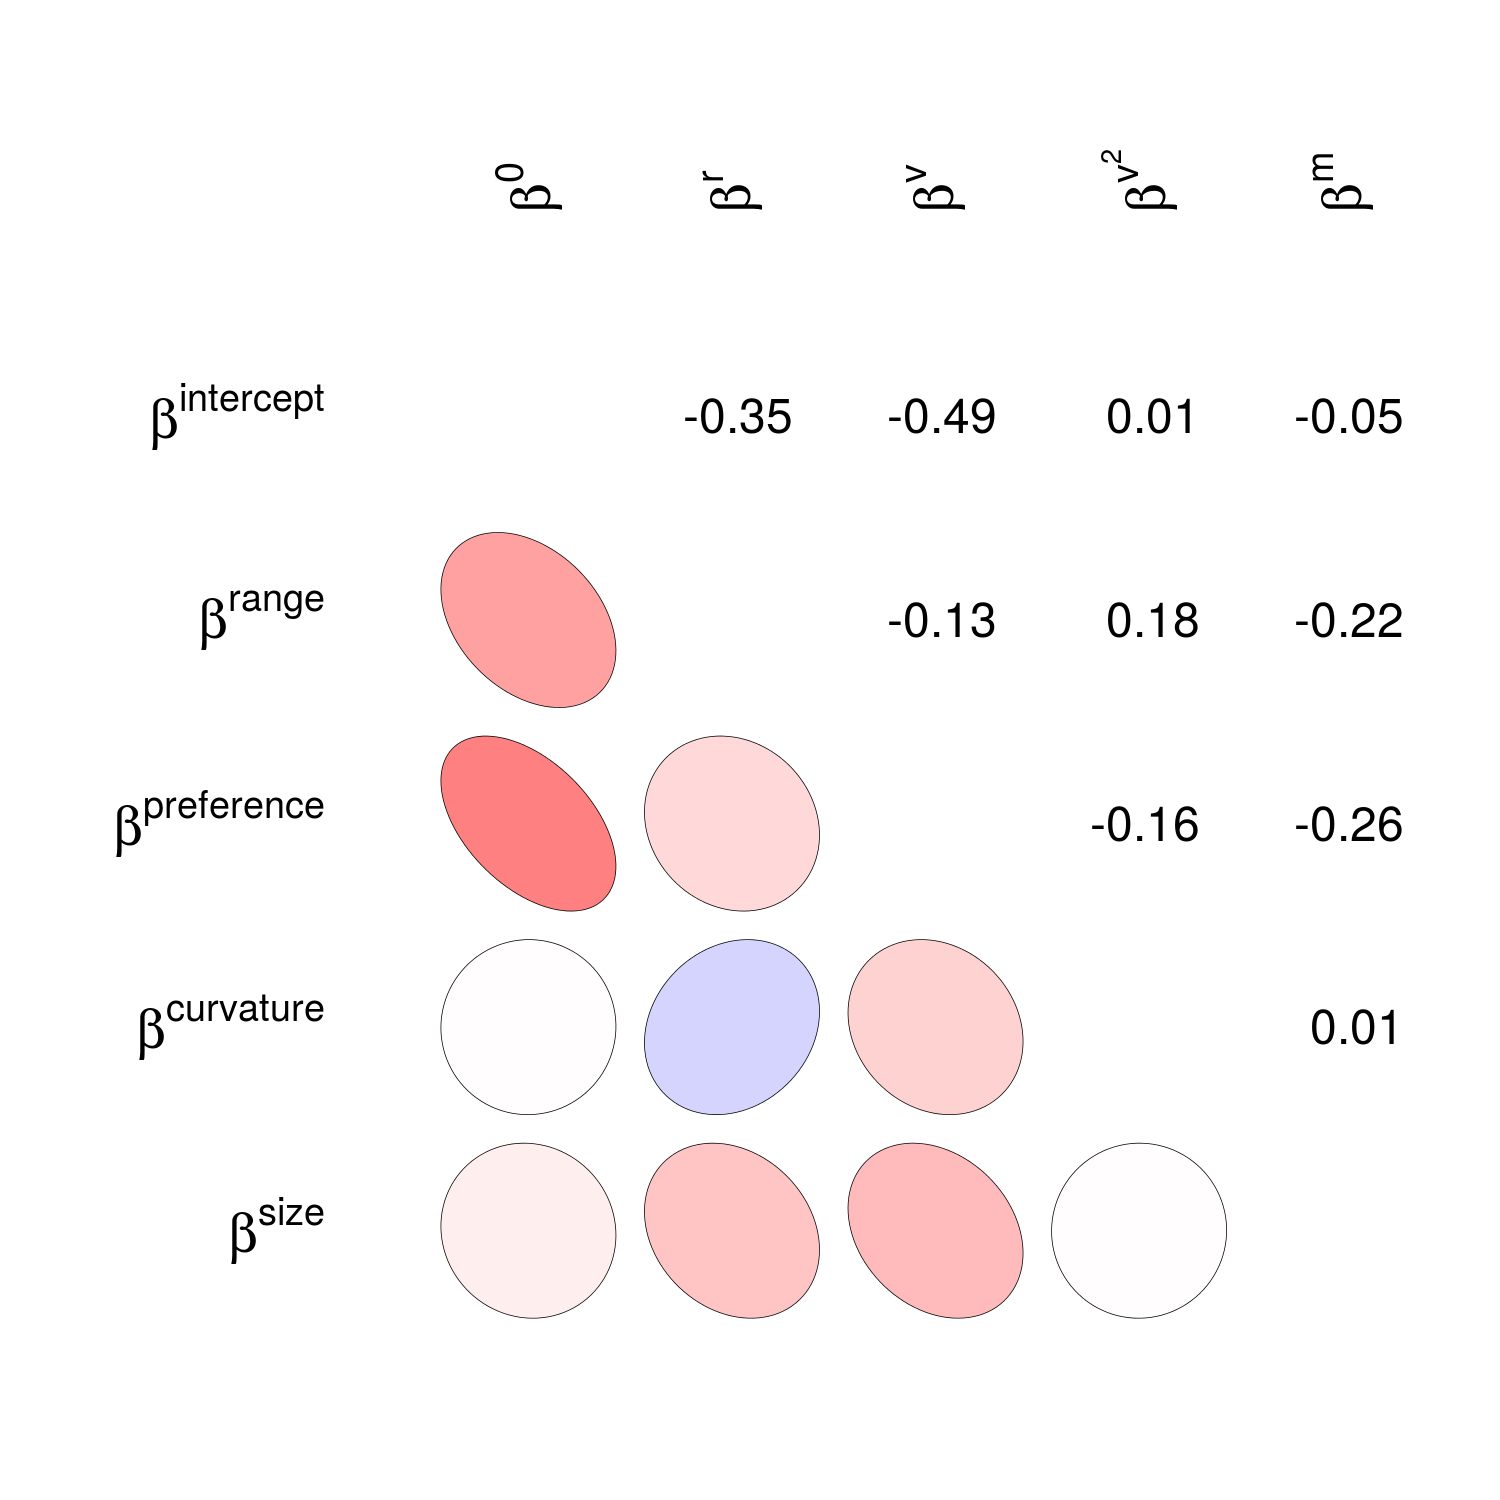
\includegraphics[width = \textwidth,height = 0.9\textheight,keepaspectratio = true]{figure/wei_cor_heatmap}
  \end{center}
\end{frame}

\begin{frame}
  \begin{block}{Summary of results}
    \begin{itemize}
      \item Effect of geographic range consistent with prior expectations; low variance.
      \item No effect of body size; low variance.
      \item Epicontinental environmental preference slightly favored on averaged; high variance. 
      \item Strong support for survival of unspecialized as generalization wrt environmental preference; medium variance.
    \end{itemize}
  \end{block}
\end{frame}

\begin{frame}
  \begin{alertblock}{Macroevolutionary process}
    \begin{itemize}
      \item Magnitude of effect of geographic range and environmental preference increase with extinction intensity.
      \item As extinction risk decreases, the differences between taxa matter less.
      \item Evidence for qualitative difference between mass and background extinction.
    \end{itemize}
  \end{alertblock}
\end{frame}



\section{Patterns in functional diversity}

\begingroup
\AtBeginSubsection{}

\subsection{Mammal species pool functional composition}

\begin{frame}
  \begin{alertblock}{Question}
    When are certain ecologies, ecotypes, or functional groups enriched or depleted in a species pool?
  \end{alertblock}
\end{frame}

\begin{frame}
  \frametitle{Age of Mammals}
  \begin{center}
    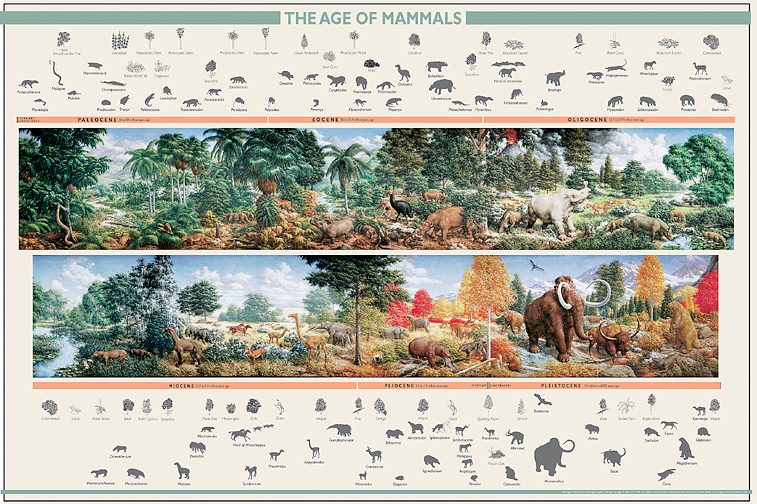
\includegraphics[width = \textwidth,height = 0.8\textheight,keepaspectratio = true]{figure/aom}
  \end{center}
\end{frame}

\begin{frame}
  \begin{center}
    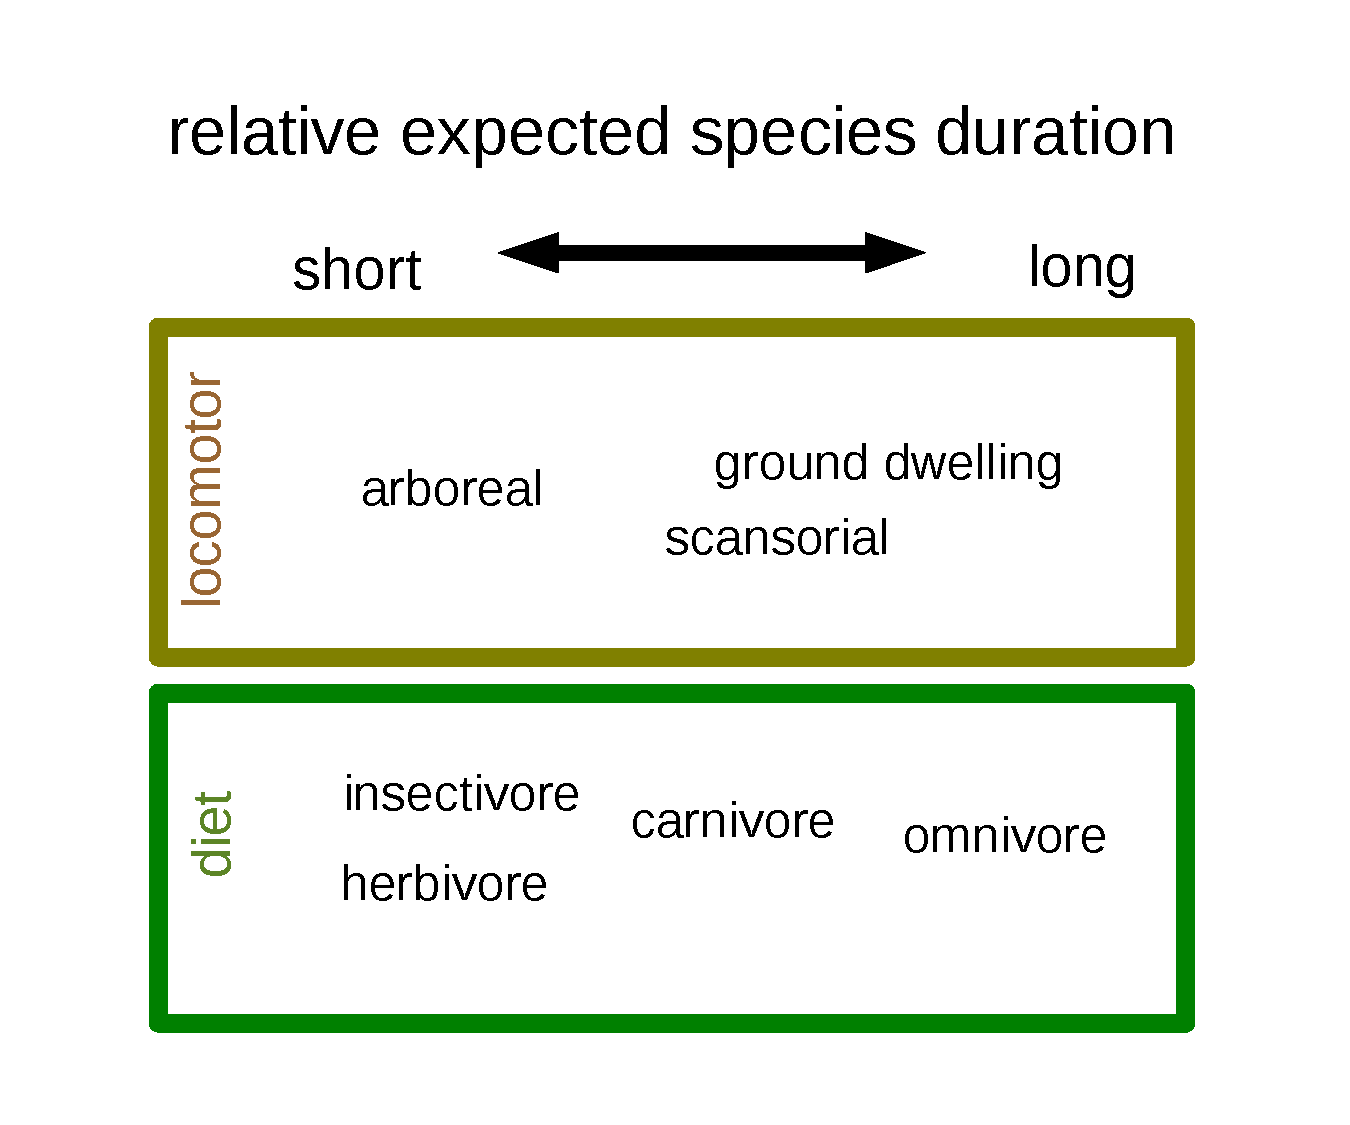
\includegraphics[height=0.8\textheight,width=\textwidth,keepaspectratio=true]{figure/smits_2015_results}
  \end{center}

  \tiny{\attrib{Smits 2015 \em{PNAS}}}
\end{frame}

\begin{frame}
  \frametitle{Fourth-corner modelling problem}
  \begin{center}
    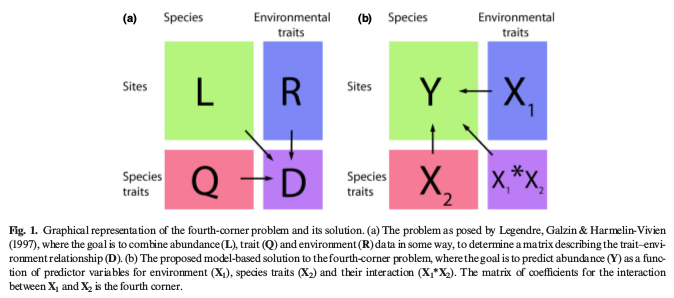
\includegraphics[height=0.8\textheight,width=\textwidth,keepaspectratio=true]{figure/brown_fourth_corner}
  \end{center}

  \tiny{\attrib{Brown \em{et al.} 2014 \em{Methods Ecol. Evol.}}}
\end{frame}

\begin{frame}
  \frametitle{Covariates of interest}
  \begin{columns}
    \begin{column}{0.5\textwidth}
      individual-level \\(species i at time unit t)
      \begin{itemize}
        \item ecotype: combination diet and locomotor categories
          \begin{itemize}
            \item effect is function of group-level covariates
          \end{itemize}
        \item body size \\(rescaled log body mass)
      \end{itemize}
    \end{column}
    \begin{column}{0.5\textwidth}
      group-level (2 My time unit t)
      \begin{itemize}
        \item temperature record based on Mg/Ca estimates
          \begin{itemize}
            \item mean and range \\(rescaled log degrees)
          \end{itemize}
        \item plant community phase following Graham 2011
      \end{itemize}
    \end{column}
  \end{columns}
\end{frame}

\begin{frame}
  \frametitle{Paleontological fourth-corner model}
  \begin{center}
    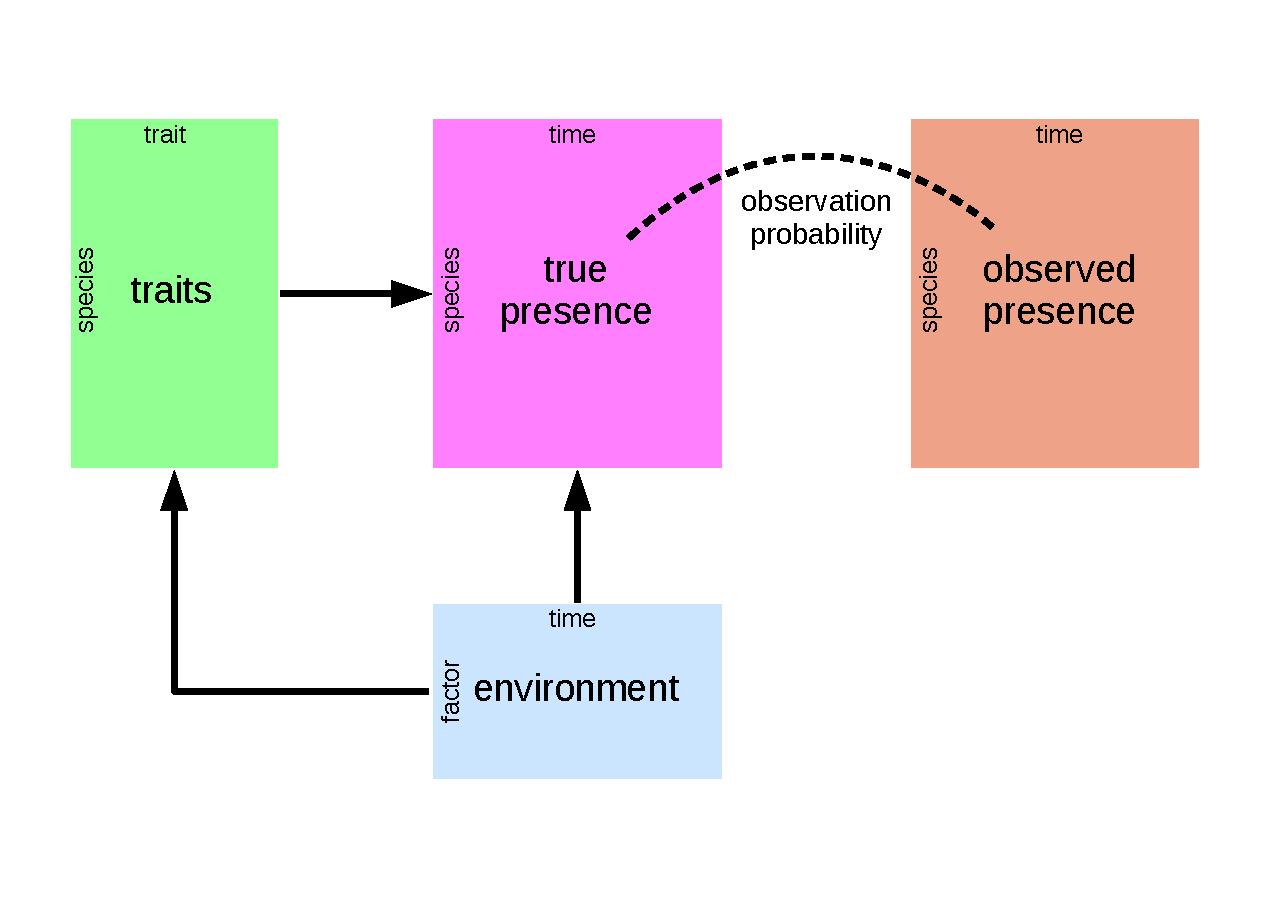
\includegraphics[height=0.8\textheight,width=\textwidth,keepaspectratio=true]{figure/paleo_fourth_corner}
  \end{center}

\end{frame}

\begin{frame}
  \frametitle{Model and sampling statement definition}
  \begin{center}
    \begin{scriptsize}
      \begin{columns}
        \begin{column}{0.5\textwidth}
          \begin{align*}
            y_{i, t} &\sim \text{Bernoulli}(p_{i, t} z_{i, t}) \\
            p_{i, t} &= \text{logit}^{-1}(\alpha_{0} + \alpha_{1} m_{i} + r_{t}) \\ 
            r_{t} &\sim \mathcal{N}(0, \sigma) \\
            \alpha_{0} &\sim \mathcal{N}(0, 1) \\
            \alpha_{1} &\sim \mathcal{N}(1, 1) \\
            \sigma &\sim \mathcal{N}^{+}(1) \\
            z_{i, 1} &\sim \text{Bernoulli}(\phi_{i, 1}) \\
            z_{i, t} &\sim \text{Bernoulli}\left(z_{i, t - 1} \pi_{i,t} + \sum_{x = 1}^{t}(1 - z_{i, x}) \phi_{i,t}\right) \\
            \phi_{i, t} &= \text{logit}^{-1}(a^{\phi}_{t, j[i]} + b^{\phi}_{1} m_{i} + b^{\phi}_{2} m_{i}^{2}) \\
            \pi_{i, t} &= \text{logit}^{-1}(a^{\pi}_{t, j[i]} + b^{\pi}_{1} m_{i} + b^{\pi}_{2} m_{i}^{2}) \\
            a^{\phi} &\sim \text{MVN}(U \gamma^{\phi}, \Sigma^{\phi}) \\
            a^{\pi} &\sim \text{MVN}(U \gamma^{\pi}, \Sigma^{\pi}) \\
          \end{align*}
        \end{column}
        \begin{column}{0.5\textwidth}
          \begin{align*}
            \Sigma^{\phi} &= \text{diag}(\tau^{\phi}) \Omega^{\phi} \text{diag}(\tau^{\phi}) \\
            \Sigma^{\pi} &= \text{diag}(\tau^{\pi}) \Omega^{\pi} \text{diag}(\tau^{\pi}) \\
            \rho &\sim \text{U}(0, 1) \\
            b^{\phi}_{1} &\sim \mathcal{N}(0, 1) \\
            b^{\pi}_{1} &\sim \mathcal{N}(0, 1) \\
            b^{\phi}_{2} &\sim \mathcal{N}(-1, 1) \\
            b^{\pi}_{2} &\sim \mathcal{N}(-1, 1) \\
            \gamma^{\phi} &\sim \mathcal{N}(0, 1) \\
            \gamma^{\pi} &\sim \mathcal{N}(0, 1) \\
            \tau^{\phi} &\sim \mathcal{N}^{+}(1) \\
            \tau^{\pi} &\sim \mathcal{N}^{+}(1) \\
            \Omega^{\phi} &\sim \text{LKJ}(2) \\
            \Omega^{\pi} &\sim \text{LKJ}(2). \\
          \end{align*}
        \end{column}
      \end{columns}
    \end{scriptsize} 
  \end{center}
\end{frame}



%\begin{frame}
%  \frametitle{Posterior predictive performance}
%
%  \begin{columns}
%    \begin{column}{0.5\textwidth}
%      \begin{center}
%        Pure-presence
%
%        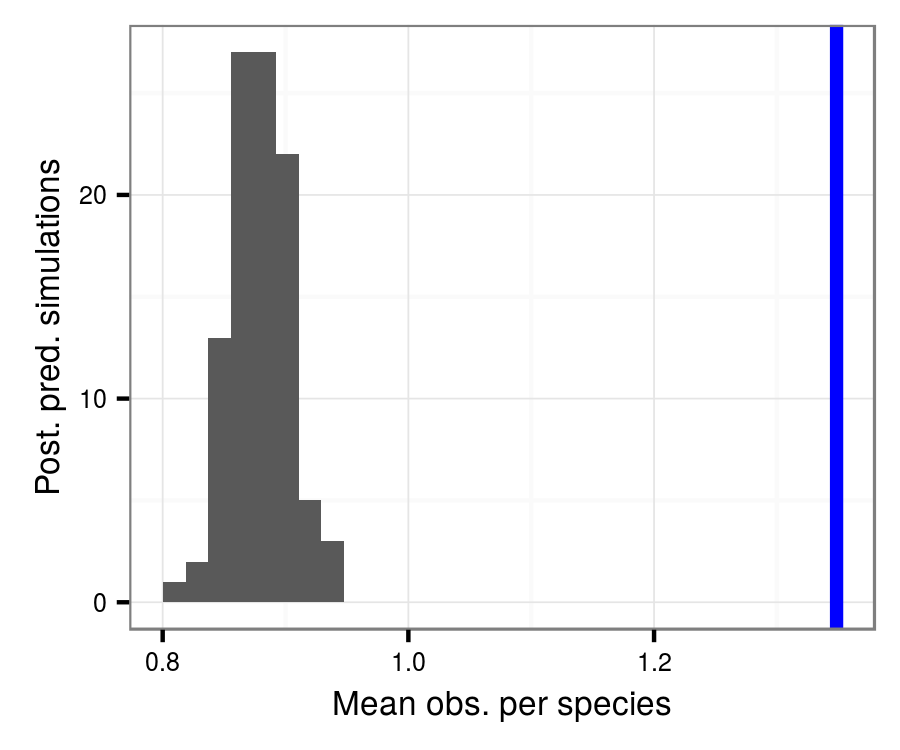
\includegraphics[height=0.8\textheight,width=\textwidth,keepaspectratio=true]{figure/pred_occ}
%      \end{center}
%    \end{column}
%    \begin{column}{0.5\textwidth}
%      \begin{center}
%        Birth-death 
%
%        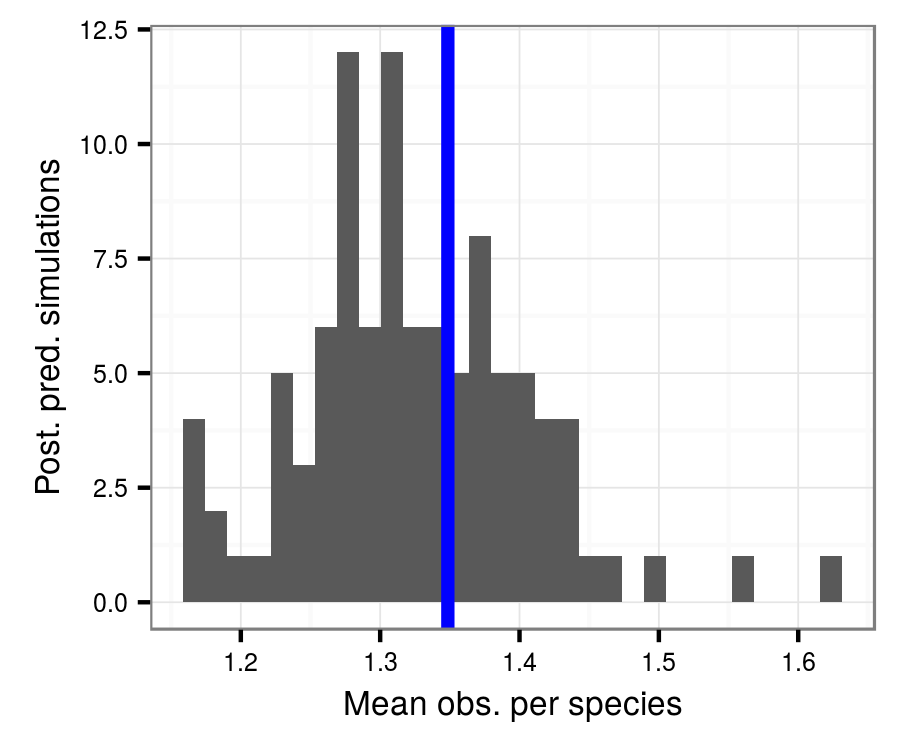
\includegraphics[height=0.8\textheight,width=\textwidth,keepaspectratio=true]{figure/pred_occ_bd}
%      \end{center}
%    \end{column}
%  \end{columns}
%\end{frame}

\begin{frame}
  \frametitle{Probability of ecotype origination}
  \begin{center}
    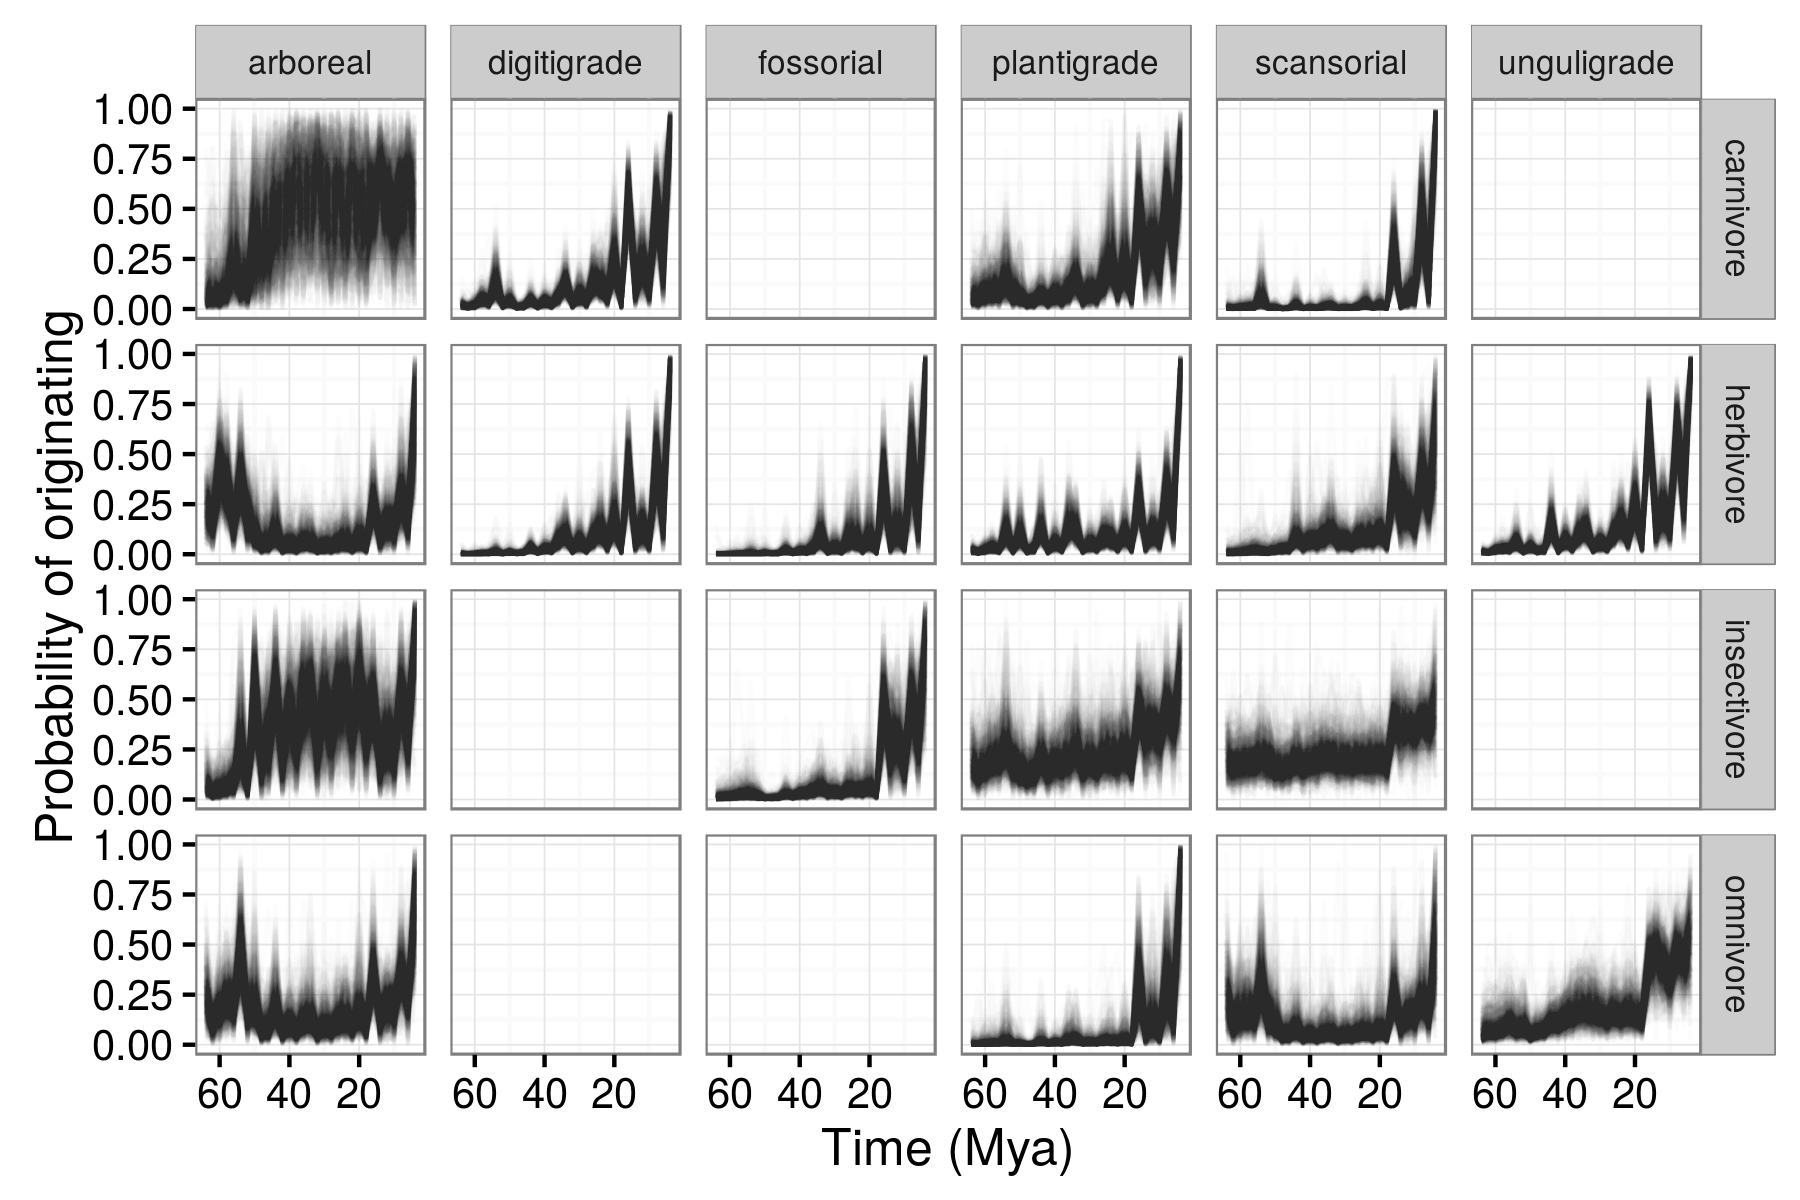
\includegraphics[height=0.8\textheight,width=\textwidth,keepaspectratio=true]{figure/ecotype_origin_bd}
  \end{center}
\end{frame}

\begin{frame}
  \frametitle{Probability of ecotype survival}
  \begin{center}
    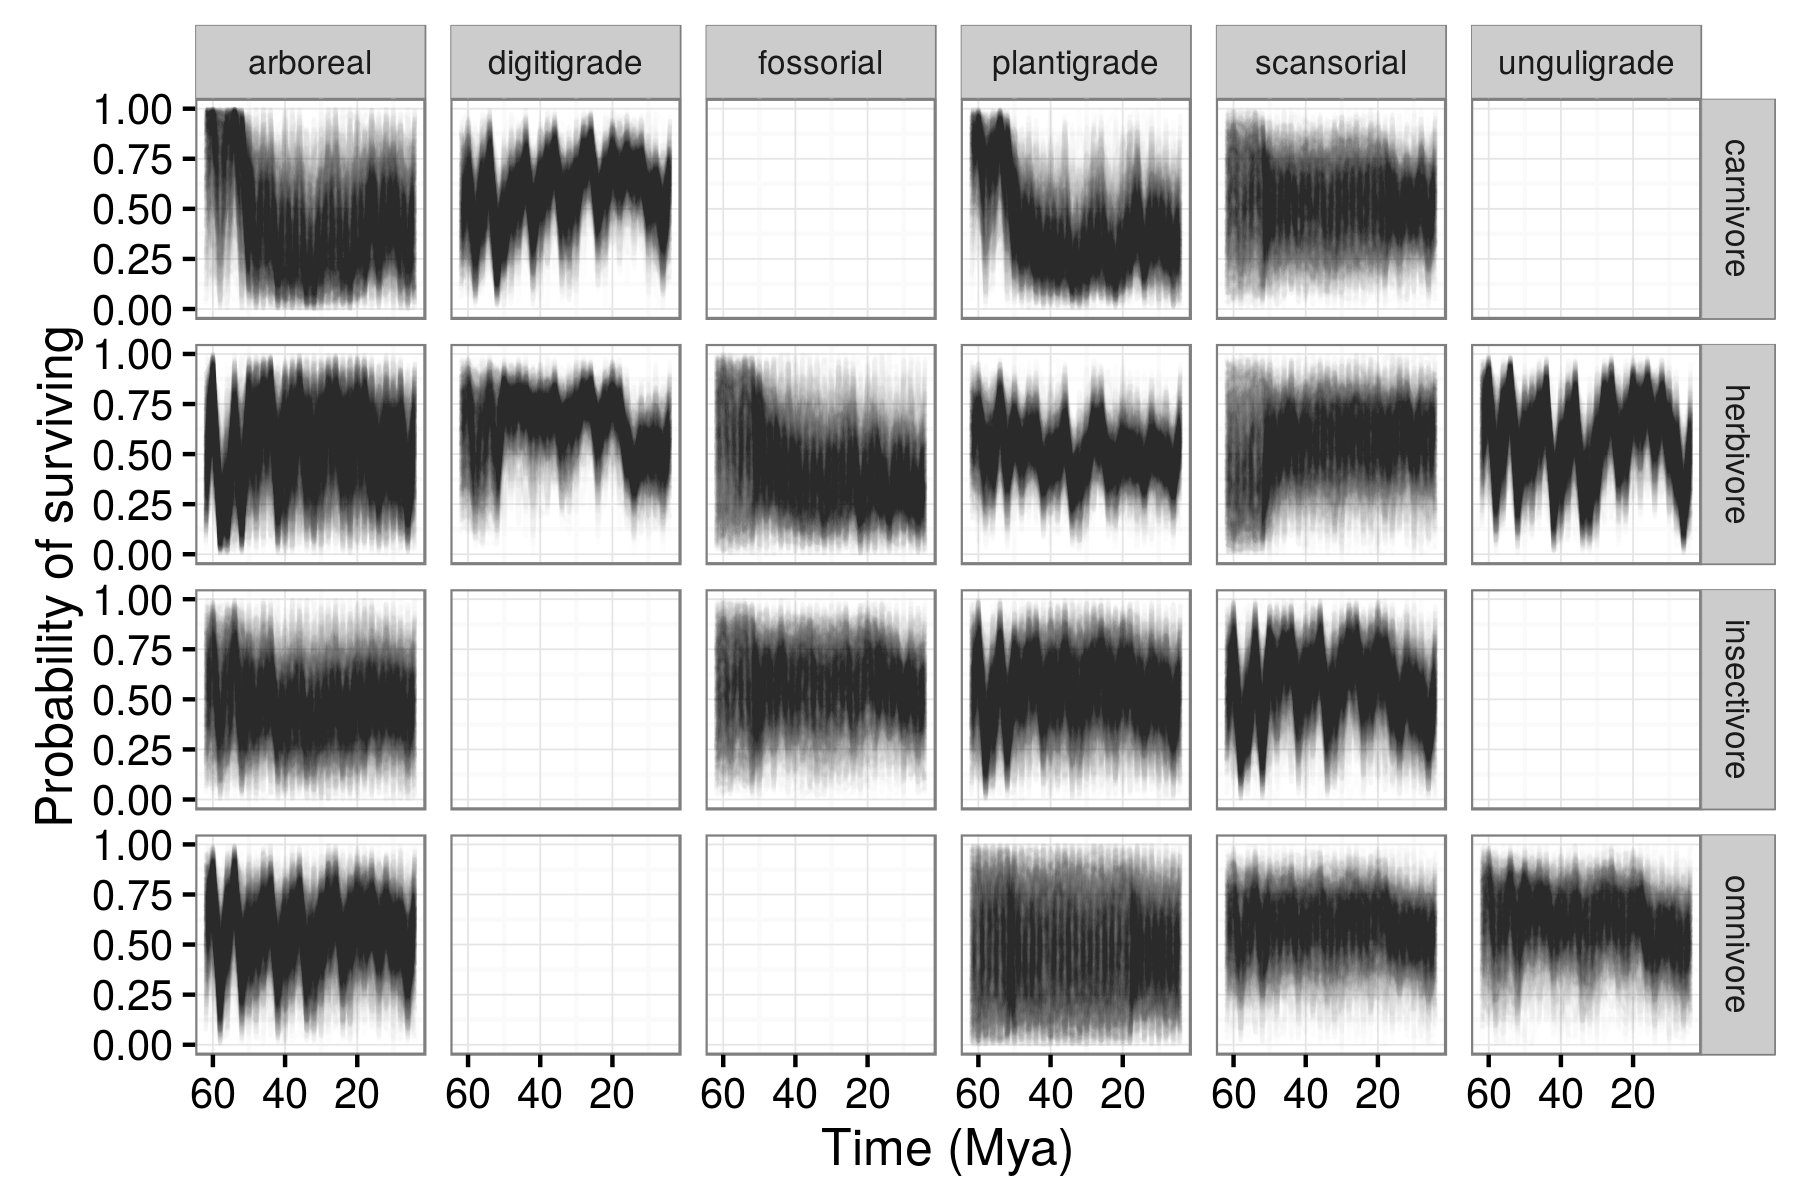
\includegraphics[height=0.8\textheight,width=\textwidth,keepaspectratio=true]{figure/ecotype_survival_bd}
  \end{center}
\end{frame}

\begin{frame}
  \frametitle{Group-level effects (plant phase, climate) on origination}
  \begin{center}
    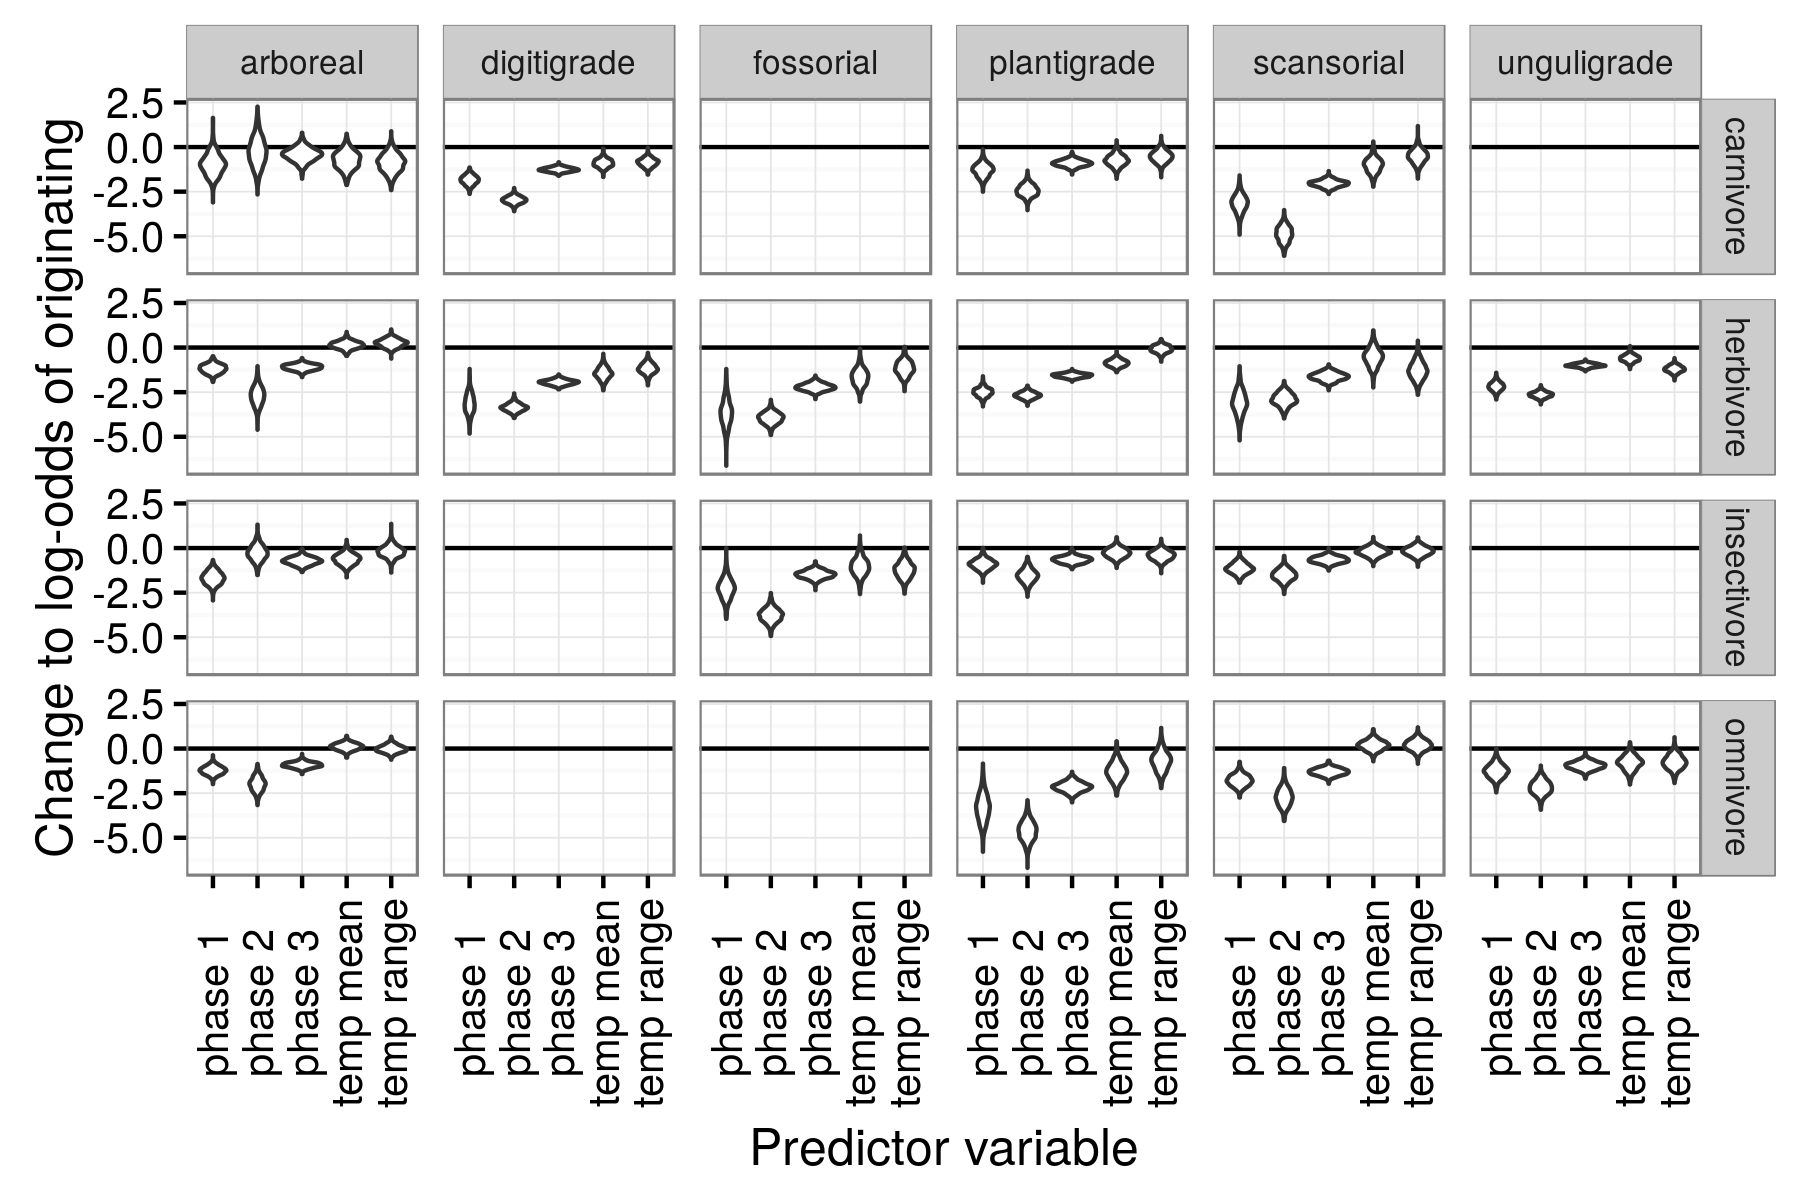
\includegraphics[height=0.8\textheight,width=\textwidth,keepaspectratio=true]{figure/group_on_origin_bd}
  \end{center}
\end{frame}

\begin{frame}
  \frametitle{Group-level effects (plant phase, climate) on survival}
  \begin{center}
    \includegraphics[height=0.8\textheight,width=\textwidth,keepaspectratio=true]{figure/group_on_survival_bd}
  \end{center}
\end{frame}

\begin{frame}
  \frametitle{Total species pool diversity and diversification}
  \begin{columns}
    \begin{column}{0.5\textwidth}
      \begin{center}
        \includegraphics[height=0.4\textheight,width=\textwidth,keepaspectratio=true]{figure/log_diversity}

        \includegraphics[height=0.4\textheight,width=\textwidth,keepaspectratio=true]{figure/orig_rate}
      \end{center}
    \end{column}
    \begin{column}{0.5\textwidth}
      \begin{center}
        \includegraphics[height=0.4\textheight,width=\textwidth,keepaspectratio=true]{figure/div_rate}

        \includegraphics[height=0.4\textheight,width=\textwidth,keepaspectratio=true]{figure/death_rate}
      \end{center}
    \end{column}
  \end{columns}
\end{frame}

\begin{frame}
  \frametitle{Ecotype-specific diversity}
  \begin{center}
    \includegraphics[height=0.8\textheight,width=\textwidth,keepaspectratio=true]{figure/ecotype_diversity}
  \end{center}
\end{frame}

%\begin{frame}
%  \frametitle{Ecotype-specific origination}
%  \begin{center}
%    \includegraphics[height=0.8\textheight,width=\textwidth,keepaspectratio=true]{figure/birth_eco}
%  \end{center}
%\end{frame}
%
%\begin{frame}
%  \frametitle{Ecotype-specific extinction}
%  \begin{center}
%    \includegraphics[height=0.8\textheight,width=\textwidth,keepaspectratio=true]{figure/death_eco}
%  \end{center}
%\end{frame}

\begin{frame}
  \frametitle{Relative ecotype diversity}
  \begin{center}
    \includegraphics[height=0.8\textheight,width=\textwidth,keepaspectratio=true]{figure/relative_diversity}
  \end{center}
\end{frame}

\begin{frame}
  \begin{block}{Summary of results}
    \begin{itemize}
      \item changes to ecotype composition driven by origination, not extinction
        \begin{itemize}
          \item specific ecotypes source of most variation in overall origination
        \end{itemize}
      \item arboreal taxa decrease through Paleogene, all but absent by Neogene
      \item digitigrade and unguligrade herbivores only groups with sustained increase
      \item environmental covariates virtually always affect origination, not survival
    \end{itemize}
  \end{block}
\end{frame}


\endgroup


\section{Conclusions and commentary}
\begin{frame}
  \frametitle{High level overview}
  \begin{itemize}
    \item<1-> macroevolution and macroecology devoted to explaining emergent patterns in evolution and ecology
    \item<2-> emphasis on functional traits yields strong and intuitive results because of obvious selective importance
    \item<3-> Gelman: ``big data are messy. messy data need large models. large models need Bayesian inference.''
  \end{itemize}
\end{frame}

\begin{frame}
  \frametitle{Synthesis}

  \begin{itemize}
    \item<1-> \alert{law of constant extinction}
      \begin{itemize}
        \item neither study of survival supports this
        \item evidence instead for increasing risk with duration
      \end{itemize}
    \item<2-> \alert{survival of the unspecialized}
      \begin{itemize}
        \item strong support as generality; should be our ``null''
        \item brachiopods: when extinction intensity high this pattern breaks
          \begin{itemize}
            \item qualitative difference between mass and background extinction
          \end{itemize}
      \end{itemize}
    \item<3-> \alert{functional diversity}
      \begin{itemize}
        \item hypotheses from macroevolution can inspire macroecological study
        \item model unifies macroevolutionary and macroecological frameworks
      \end{itemize}
  \end{itemize}
\end{frame}


%\begin{frame}
%  \begin{center}
%    \huge{\uppercase{final thoughts}}
%  \end{center}
%\end{frame}



\begin{frame}
  \frametitle{Acknowledgements}
  \begin{center}
    \includegraphics[width=0.45\textwidth,height=0.4\textheight,keepaspectratio=true]{figure/committee/ken}
    \includegraphics[width=0.45\textwidth,height=0.4\textheight,keepaspectratio=true]{figure/committee/foote}

    \includegraphics[width=0.33\textwidth,height=0.4\textheight,keepaspectratio=true]{figure/committee/david_2}
    \includegraphics[width=0.33\textwidth,height=0.4\textheight,keepaspectratio=true]{figure/committee/rick}
    \includegraphics[width=0.33\textwidth,height=0.4\textheight,keepaspectratio=true]{figure/committee/graham}
  \end{center}
\end{frame}

\begin{frame}
  \frametitle{Acknowledgements}
  \begin{center}
    \includegraphics[width=\textwidth,height=0.1\textheight,keepaspectratio=true]{figure/ceb}
  \end{center}

  \begin{columns}
    \begin{column}{0.35\textwidth}
      \begin{itemize}
        \item \tiny{Angielczyk lab}
          \begin{itemize}
            \item \tiny{David Grossnickle, Dallas Krentzel, Jackie Lungmus, Jonathan Mitchell}
          \end{itemize}
        \item \tiny{Foote lab}
          \begin{itemize}
            \item \tiny{Marites Villarosa Garcia, Samuel Miller, Nadia Pierrehumbert, Kathleen Ritterbush}
          \end{itemize}
        \item \tiny{Gregory Wilson}
        \item \tiny{Alistair Evans}
        \item \tiny{Jeff Bradley, Donald Grayson, Jim Kenagy, Nancy Simmons}
        \item \tiny{Sandy Carlson, Christine Janis}
      \end{itemize}
    \end{column}
    \begin{column}{0.35\textwidth}
      \begin{itemize}
        \item \tiny{Carolyn Johnson, \\Elizabeth Eakin}
        \item \tiny{2012 CEB cohort, 2012 Paleo cohort}
        \item \tiny{\alert{Stewart Edie}, Amy Henry, Katherine Silliman, Sarah Tulga, Max Winston}
        \item \tiny{\alert{Ben Frable}, Brian Goodrich, Colin Kyle, \alert{Darcy Ross}, Elizabeth Sander, Laura Southcott, \alert{Julie Symaszek}, Brian Waligorski}
        \item \tiny{Jean Leahy}
      \end{itemize}
    \end{column}
    \begin{column}{0.25\textwidth}
      \includegraphics[width=\textwidth,height=\textheight,keepaspectratio=true]{figure/paleodb}
    \end{column}
  \end{columns}
\end{frame}

\begin{frame}
  \frametitle{Acknowledgements}
  \centering
  \includegraphics[width=0.33\textwidth,height=\textheight,keepaspectratio=true]{figure/family/lex_timmy_anniversary_edit}
  \includegraphics[width=0.33\textwidth,height=\textheight,keepaspectratio=true]{figure/family/james_edit}
  \includegraphics[width=0.33\textwidth,height=\textheight,keepaspectratio=true]{figure/family/megan_1_edit}
\end{frame}


\end{document}
